
%\ctparttext{\color{black}
%    \begin{center}
%
%    \end{center}
%}

\newpage
\blankpage

\ctparttext{
  \color{black}
  \begin{center}
    \textit{Las matemáticas son el único material didáctico que se puede presentar de una manera totalmente no dogmática. (Max Dehn)}
  \end{center}
}


\part{Parte informática}

%\part{Librería en Python}
\chapter{Librería en Python}




\section{Introducción}




\iffalse
Sea $G$ un grupo definido por una presentación finita $\langle X \mid R \rangle $. Como se ha comentado anteriormente, el problema de palabras \textit{(word problem)} para el grupo $G$ cuestiona si existe un algoritmo para determinar si una palabra en $X^{\pm 1}$ representa el elemento identidad de $G$ o, equivalentemente, determinar si dos palabras generan el mismo elemento.  Fueron \textit{Nivikov} y \textit{Boone} quieres demostraron que se trataba de un problema indecidible y mostraron la existencia de grupos con presentación finita en el que no existía dicho algoritmo. 

Es importante destacar que aunque no haya un algoritmo general para resolver el problema de palabras dado un conjunto arbitrario de generadores y relatores, en muchos casos de grupos finitos se puede resolver mediante una técnica llamada enumeración de clases (\textit{coset enumeration}).

En teoría de grupos, la enumeración de clases es el problema de contar las clases de un subgrupo $H$ de un grupo $G$ dado en términos de una presentación.
En $1936$, \textit{J.A. Todd} y \textit{H.S.M. Coxeter} describieron el algoritmo original, que se caracterizaba por ser un método bastante mecánico enfocado para realizarse manualmente. Sin embargo, y debido a su complejidad, se convirtió en uno de los primeros algoritmos del área de las matemáticas en hacer uso de los ordenadores electrónicos cuando estos estuvieron disponibles.
\fi







%Con el inicio de la Teoría de grupos en los siglos \texttt{XVIII}. y \texttt{XIX}, muchos matemáticos influyentes fundamentaron los conceptos relacionados con grupos. Destacamos a 
 Walter Von Dyck es considerado el precursor de la Teoría Combinatoria de Grupos tras sus trabajos sobre la construcción de grupo libre y definición de grupo dado por generadores y relatores. A raíz de sus estudios, en 1911, el matemático Max Dehn publicó un artículo con la formulación de los tres problemas de decisión más conocidos en Teoría de Grupos: El Problema de Palabras, Conjugación e Isomorfismo.

\begin{enumerate}
    \item El Problema de Conjugación para un grupo es el problema de decisión de determinar si dos elementos $x, y \in G$ son elementos conjugados o no; es decir, si existe $z\in G$ que cumpla $x=zyz^{-1}$. Este problema se conoce también como Problema de la Transformación.
    
    \item El Problema del Isomorfismo para dos grupos es el problema de decidir si son isomorfos o no.
    
    \item El Problema de Palabras para grupos finitamente generados es el problema algorítmico de decidir si dos palabras dadas como producto de generadores representan el mismo elemento. Nos centraremos principalmente en este.
\end{enumerate}

Un año más tarde, en 1912, Dehn dio un algoritmo capaz de resolver el Problema de Conjugación y Palabras para grupos definidos con una única relación. Sin embargo, pasaron años hasta que estos problemas fueron resueltos, siendo muchos los matemáticos quienes poco a poco presentaban soluciones para algunos grupos específicos, sin obtener unos avances importantes. En 1936, J.A. Todd y H.S.M. Coxeter describieron un algoritmo capaz de resolver el Problema de Palabras, el \textit{Algoritmo de Todd Coxeter}, que debido a su complejidad, no se podía ejecutar sobre cualquier grupo.

Así fue hasta la llegada de Alang Turing, el primer matemático e informático que logró formalizar los conceptos de algoritmo y computación. De hecho, es considerado el padre de la computación por todos sus aportes sobre inteligencia artificial, el más importante vino en 1945, el diseño en detalle del primer ordenador.

Con la llegada de los primeros ordenadores electrónicos, muchos matemáticos no dudaron en aprovechar las ventajas que supondrían para sus estudios. Especialmente, los algebraicos vieron como el estudio de nuevos grupos creció inimaginablemente, expandiéndose de una forma nunca antes vista.

A raíz de este origen, se dirigieron muchas investigaciones para promover el estudio de grupos mediante ayuda de ordenadores. 
Una de las primeras y más importantes fue dirigida en $1951$, donde M.H.A. Newman motivó la investigación de todos los grupos de orden hasta $256$. En relación con el \textit{Algoritmo de Todd Coxeter}, surgieron las primeras implementaciones a ordenador del algoritmo original y a día de hoy hasta existen algoritmos que pueden resolver el Problema de Palabras en grupos de orden infinito, como es el caso del \textit{Algoritmo de Knuth-Bendix} ~\cite{knuth}.




Nuestro trabajo consistirá en la extensión y optimización de la librería de Teoría de Grupos de José L. Bueso Montero y Pedro A. García Sánchez, basada en la librería de Naftali Harris y disponible en ~\cite{Pedrito} y ~\cite{Absalg}, respectivamente. Esta librería se presenta como un recurso didáctico, complementario y de profundización de la teoría algebraica estudiada durante la carrera. Está disponible en \href{https://github.com/lmd-ugr/Grupos}{github.com/lmd-ugr/Grupos},  y para facilitar su uso, se ha proporcionado un tutorial en Jupyter.


El primer paso realizado fue el estudio teórico de todos los ficheros y métodos programados, donde se anotaron todos los posibles cambios para su modificación posterior. Originalmente, los ficheros eran los siguientes:

\begin{itemize}
    \item \texttt{Set.py}: contiene la clase para definir un conjunto \textit{Set} de tipo \textit{frozenset} (para que éste sea inmutable). Este conjunto contendrá los elementos de un grupo, que tendrán un carácter estático, es decir, no se podrán modificar una vez creados.
    
    \item \texttt{Function.py}: la clase \textit{Function} simulará la operación binaria del grupo. Su dominio y codominio son conjuntos de tipo \textit{Set} y contiene métodos para comprobar la inyectividad, sobreyectividad y biyectividad de la función.
    
    \item \texttt{Group.py}: contiene la principal clase de la librería, la clase Grupo. En ella, se le da estructura de grupo a un conjunto de tipo \textit{Set} junto a su operación binaria \textit{Function}. Su constructor se encarga de comprobar que se cumplen los axiomas de grupo (asociatividad, existencia de elemento neutro y existencia de inverso para cada elemento) y contiene métodos que abarcan los principales conceptos de la asignatura Álgebra II.
\end{itemize}

La librería únicamente permitía la construcción de un grupo dando un conjunto de elementos junto a una operación binaria (o tabla de multiplicar) que satisfagan los axiomas de grupo.  Para grupos de orden pequeño esto no supone un gran problema, sin embargo, definir un grupo de orden elevado de esta forma no es recomendable ya que puede llegar a ser muy ineficiente. Por esta razón, se han creado nuevas clases para representar los diferentes grupos, donde se han sobrecargado los métodos que definen cada una de sus operaciones binarias. %Además, se ha completado la documentación de cada método y función implementada. %De esta forma, no haría falta indicar la tabla de multiplicar.

Además, se ha realizado la implementación del \textit{Algoritmo de Todd Coxeter}. Así, podremos definir grupos dados en términos de generadores y relatores y obtener su representación por permutaciones, a los que aplicaremos diferentes métodos para identificarlos, mediante isomorfismos, con grupos conocidos. Véase la Sección \ref{TC} para una descripción detallada del algoritmo.



\section{Optimización}



En esta sección se comentarán los cambios realizados en cada
clase de la librería, que se han implementado siguiendo los conceptos matemáticos descritos anteriormente. Además, se ha completado y añadido la documentación de cada método y función implementada, por lo que el usuario puede consultarla si así lo desea. \\
Se usará Jupyter para ilustrar algunos ejemplos, donde únicamente bastará con importar la librería que queramos para poder usar todos sus métodos implementados.

\begin{itemize}

\item \texttt{Set.py}: se han añadido métodos para realizar operaciones
  a nivel de conjunto.

  \begin{itemize}
  \item Unión, diferencia, intersección, producto cartesiano y diferencia
    simétrica.


    \begin{tcolorbox}[breakable, size=fbox, boxrule=1pt, pad at break*=1mm,colback=cellbackground, colframe=cellborder]
\prompt{In}{incolor}{1}{\boxspacing}
\begin{Verbatim}[commandchars=\\\{\}]
\PY{k+kn}{from} \PY{n+nn}{Set} \PY{k+kn}{import} \PY{n}{Set}
\end{Verbatim}
\end{tcolorbox}

    
    \begin{tcolorbox}[breakable, size=fbox, boxrule=1pt, pad at break*=1mm,colback=cellbackground, colframe=cellborder]
\prompt{In}{incolor}{2}{\boxspacing}
\begin{Verbatim}[commandchars=\\\{\}]
\PY{n}{A} \PY{o}{=} \PY{n}{Set}\PY{p}{(}\PY{p}{\PYZob{}}\PY{l+m+mi}{1}\PY{p}{,}\PY{l+m+mi}{2}\PY{p}{,}\PY{l+m+mi}{3}\PY{p}{\PYZcb{}}\PY{p}{)}
\PY{n}{B} \PY{o}{=} \PY{n}{Set}\PY{p}{(}\PY{p}{\PYZob{}}\PY{l+m+mi}{2}\PY{p}{,}\PY{l+m+mi}{4}\PY{p}{\PYZcb{}}\PY{p}{)}
\end{Verbatim}
\end{tcolorbox}


    \begin{tcolorbox}[breakable, size=fbox, boxrule=1pt, pad at break*=1mm,colback=cellbackground, colframe=cellborder]
\prompt{In}{incolor}{3}{\boxspacing}
\begin{Verbatim}[commandchars=\\\{\}]
\PY{n}{C} \PY{o}{=} \PY{n}{A}\PY{o}{*}\PY{n}{B}
\PY{n}{C}
\end{Verbatim}
\end{tcolorbox}


    \begin{tcolorbox}[breakable, size=fbox, boxrule=.5pt, pad at break*=1mm, opacityfill=0]
\prompt{Out}{outcolor}{3}{\boxspacing}
\begin{Verbatim}[commandchars=\\\{\}]
\{(2, 4), (1, 2), (3, 4), (2, 2), (3, 2), (1, 4)\}
\end{Verbatim}
\end{tcolorbox}
        

  

    \item \textit{cardinality}, \textit{is\_finite}: se tratan de métodos que sirven para calcular la cardinalidad del conjunto y comprobar si este es finito, respectivamente.


    \begin{tcolorbox}[breakable, size=fbox, boxrule=1pt, pad at break*=1mm,colback=cellbackground, colframe=cellborder]
\prompt{In}{incolor}{4}{\boxspacing}
\begin{Verbatim}[commandchars=\\\{\}]
\PY{n}{C}\PY{o}{.}\PY{n}{is\PYZus{}finite}\PY{p}{(}\PY{p}{)}\PY{p}{,} \PY{n}{C}\PY{o}{.}\PY{n}{cardinality}\PY{p}{(}\PY{p}{)}
\end{Verbatim}
\end{tcolorbox}

    \begin{tcolorbox}[breakable, size=fbox, boxrule=.5pt, pad at break*=1mm, opacityfill=0]
\prompt{Out}{outcolor}{4}{\boxspacing}
\begin{Verbatim}[commandchars=\\\{\}]
(True, 6)
\end{Verbatim}
\end{tcolorbox}
        
        
    \item \textit{subsets}:  este método se encarga de calcular los subconjuntos de un conjunto. Si por parámetro se le pasa un número natural $n$, entonces calculará los subconjuntos de tamaño $n$.
    


    \begin{tcolorbox}[breakable, size=fbox, boxrule=1pt, pad at break*=1mm,colback=cellbackground, colframe=cellborder]
\prompt{In}{incolor}{5}{\boxspacing}
\begin{Verbatim}[commandchars=\\\{\}]
\PY{n}{A}\PY{o}{.}\PY{n}{subsets}\PY{p}{(}\PY{p}{)}
\end{Verbatim}
\end{tcolorbox}


\begin{tcolorbox}[breakable, size=fbox, boxrule=.5pt, pad at break*=1mm, opacityfill=0]
\prompt{Out}{outcolor}{5}{\boxspacing}
\begin{Verbatim}[commandchars=\\\{\}]
[\{1\}, \{2\}, \{3\}, \{1, 2\}, \{1, 3\}, \{2, 3\}, \{1, 2, 3\}]
\end{Verbatim}
\end{tcolorbox}
        
    \begin{tcolorbox}[breakable, size=fbox, boxrule=1pt, pad at break*=1mm,colback=cellbackground, colframe=cellborder]
\prompt{In}{incolor}{6}{\boxspacing}
\begin{Verbatim}[commandchars=\\\{\}]
\PY{n}{A}\PY{o}{.}\PY{n}{subsets}\PY{p}{(}\PY{l+m+mi}{2}\PY{p}{)}
\end{Verbatim}
\end{tcolorbox}

        \begin{tcolorbox}[breakable, size=fbox, boxrule=.5pt, pad at break*=1mm, opacityfill=0]
\prompt{Out}{outcolor}{6}{\boxspacing}
\begin{Verbatim}[commandchars=\\\{\}]
[\{1, 2\}, \{1, 3\}, \{2, 3\}]
\end{Verbatim}
\end{tcolorbox}
        
        
    \end{itemize}
  
  
\newpage
\item  \texttt{Function.py}: se ha mantenido en tu totalidad el formato
  original, a excepción del operador \textit{\_\_str\_\_} que muestra ahora
  la función de manera clara y precisa.


    \begin{tcolorbox}[breakable, size=fbox, boxrule=1pt, pad at break*=1mm,colback=cellbackground, colframe=cellborder]
\prompt{In}{incolor}{7}{\boxspacing}
\begin{Verbatim}[commandchars=\\\{\}]
\PY{k+kn}{from} \PY{n+nn}{Function} \PY{k+kn}{import} \PY{n}{Function}
\end{Verbatim}
\end{tcolorbox}

    Sea S un conjunto de tipo Set, para definir, por ejemplo, la siguiente operación binaria
    \begin{align*}
        S \times S &\rightarrow S \\
            (x,y) & \mapsto (x+y)\%3 
    \end{align*}

usaremos las función lambda que nos ofrece Python.

    \begin{tcolorbox}[breakable, size=fbox, boxrule=1pt, pad at break*=1mm,colback=cellbackground, colframe=cellborder]
\prompt{In}{incolor}{8}{\boxspacing}
\begin{Verbatim}[commandchars=\\\{\}]
\PY{n}{S} \PY{o}{=} \PY{n}{Set}\PY{p}{(}\PY{p}{\PYZob{}}\PY{l+m+mi}{0}\PY{p}{,}\PY{l+m+mi}{1}\PY{p}{,}\PY{l+m+mi}{2}\PY{p}{\PYZcb{}}\PY{p}{)}
\PY{n}{F} \PY{o}{=} \PY{n}{Function}\PY{p}{(}\PY{n}{S}\PY{o}{*}\PY{n}{S}\PY{p}{,} \PY{n}{S}\PY{p}{,}\PY{k}{lambda} \PY{n}{x}\PY{p}{:} \PY{p}{(}\PY{n}{x}\PY{p}{[}\PY{l+m+mi}{0}\PY{p}{]}\PY{o}{+}\PY{n}{x}\PY{p}{[}\PY{l+m+mi}{1}\PY{p}{]}\PY{p}{)}\PY{o}{\PYZpc{}}\PY{k}{3})
\PY{n+nb}{print}\PY{p}{(}\PY{n}{F}\PY{p}{)}
\end{Verbatim}
\end{tcolorbox}

    \begin{Verbatim}[commandchars=\\\{\}]
    f((0, 1))=1
    f((1, 2))=0
    f((2, 1))=0
    f((0, 0))=0
    f((1, 1))=2
    f((2, 0))=2
    f((0, 2))=2
    f((2, 2))=1
    f((1, 0))=1
    \end{Verbatim}

    

\item  \texttt{Group.py}:

\begin{itemize}
    \item \textit{\_\_str\_\_} y \textit{\_\_repr\_\_}: se modifican
      para además mostrar los elementos del grupo (siempre que el orden del
      grupo no sea grande).
    \item Se ha modificado el constructor \textit{\_\_init\_\_} de la clase
      \textit{Group}. De este modo, se podrán definir grupos de las dos
      formas comentadas en la Sección \ref{pg}.

  \begin{enumerate}

  \item Definición axiomatixada. Se comprueba que el par
    \textit{(Set, Function)} pasado por argumento satisface los axiomas de grupo (asociatividad, identidad e inversos).


    \begin{tcolorbox}[breakable, size=fbox, boxrule=1pt, pad at break*=1mm,colback=cellbackground, colframe=cellborder]
\prompt{In}{incolor}{9}{\boxspacing}
\begin{Verbatim}[commandchars=\\\{\}]
\PY{k+kn}{from} \PY{n+nn}{Group} \PY{k+kn}{import} \PY{o}{*}
\end{Verbatim}
\end{tcolorbox}

    
    \begin{tcolorbox}[breakable, size=fbox, boxrule=1pt, pad at break*=1mm,colback=cellbackground, colframe=cellborder]
\prompt{In}{incolor}{10}{\boxspacing}
\begin{Verbatim}[commandchars=\\\{\}]
\PY{n}{S} \PY{o}{=} \PY{n}{Set}\PY{p}{(}\PY{p}{\PYZob{}}\PY{l+m+mi}{0}\PY{p}{,}\PY{l+m+mi}{1}\PY{p}{,}\PY{l+m+mi}{2}\PY{p}{,}\PY{l+m+mi}{3}\PY{p}{\PYZcb{}}\PY{p}{)}
\PY{n}{F}\PY{o} {=} \PY{n}{Function}\PY{p}{(}\PY{n}{S}\PY{o}{*}\PY{n}{S}\PY{p}{,} \PY{n}{S}\PY{p}{,}\PY{k}{lambda} \PY{n}{x}\PY{p}{:} \PY{p}{(}\PY{n}{x}\PY{p}{[}\PY{l+m+mi}{0}\PY{p}{]}\PY{o}{+}\PY{n}{x}\PY{p}{[}\PY{l+m+mi}{1}\PY{p}{]}\PY{p}{)}\PY{o}{\PYZpc{}}\PY{k}{4})
\PY{n}{Z4} \PY{o}{=} \PY{n}{Group}\PY{p}{(}\PY{n}{S}\PY{p}{,}\PY{n}{F}\PY{p}{)}

\PY{n+nb}{print}\PY{p}{(}\PY{n}{Z4}\PY{p}{)}
\end{Verbatim}
\end{tcolorbox}

\begin{tcolorbox}[breakable, size=fbox, boxrule=.5pt, pad at break*=1mm, opacityfill=0]
\prompt{Out}{outcolor}{10}{\boxspacing}
    \begin{Verbatim}[commandchars=\\\{\}]
Group with 4 elements: \{0, 1, 2, 3\}
    \end{Verbatim}
\end{tcolorbox}

\item Definición en términos de generadores y relatores. Sea un grupo $G = \langle X \mid R\rangle$. Se pasa por argumento el conjunto de generadores $X$ y relaciones $R$ que definen al grupo. El constructor se encarga de aplicar el \textit{Algoritmo de Todd Coxeter} y darle estructura de grupo de Permutaciones al grupo $G$. Se tomará el subgrupo trivial para esta ejecución del algoritmo.


A continuación definimos el grupo $G= \langle a \mid a^4 =1 \rangle$.
    \begin{tcolorbox}[breakable, size=fbox, boxrule=1pt, pad at break*=1mm,colback=cellbackground, colframe=cellborder]
\prompt{In}{incolor}{11}{\boxspacing}
\begin{Verbatim}[commandchars=\\\{\}]
\PY{n}{gens} \PY{o}{=} \PY{p}{[}\PY{l+s+s1}{\PYZsq{}}\PY{l+s+s1}{a}\PY{l+s+s1}{\PYZsq{}}\PY{p}{]}
\PY{n}{rels} \PY{o}{=} \PY{p}{[}\PY{l+s+s1}{\PYZsq{}}\PY{l+s+s1}{aaaa}\PY{l+s+s1}{\PYZsq{}}\PY{p}{]} \PY{l+m+mi}{#a^4=1}

\PY{n}{G} \PY{o}{=} \PY{n}{Group}\PY{p}{(}\PY{n}{gensG}\PY{o}{=}\PY{n}{gens}\PY{p}{,} \PY{n}{relsG}\PY{o}{=}\PY{n}{rels}\PY{p}{)}
\PY{n+nb}{print}\PY{p}{(}\PY{n}{G}\PY{p}{)}
\end{Verbatim}
\end{tcolorbox}

    \begin{Verbatim}[commandchars=\\\{\}]
Group with 4 elements: \{(), (1, 2, 3, 4), (1, 4, 3, 2), (1, 3)(2, 4)\}
    \end{Verbatim}

Naturalmente, y aunque la forma de definir ambos grupos anteriores es distinta, son isomorfos; es
decir, $G=\langle a \mid a^4=1 \rangle \cong \mathbb{Z}_4$.

    \begin{tcolorbox}[breakable, size=fbox, boxrule=1pt, pad at break*=1mm,colback=cellbackground, colframe=cellborder]
\prompt{In}{incolor}{12}{\boxspacing}
\begin{Verbatim}[commandchars=\\\{\}]
\PY{n}{G}\PY{o}{.}\PY{n}{is\PYZus{}isomorphic}\PY{p}{(}\PY{n}{Z4}\PY{p}{)}
\end{Verbatim}
\end{tcolorbox}

\begin{tcolorbox}[breakable, size=fbox, boxrule=.5pt, pad at break*=1mm, opacityfill=0]
\prompt{Out}{outcolor}{12}{\boxspacing}
\begin{Verbatim}[commandchars=\\\{\}]
True
\end{Verbatim}
\end{tcolorbox}



Por último, se añadirá una tercera forma de definir un grupo. Sea $Y$ un conjunto de elementos, entonces el grupo $G$ se definirá como el grupo generado por $\langle Y \rangle$. En el siguiente ejemplo tomaremos un conjunto con una única permutación, sin embargo, no exigimos que los elementos sean permutaciones.
    \begin{tcolorbox}[breakable, size=fbox, boxrule=1pt, pad at break*=1mm,colback=cellbackground, colframe=cellborder]
\prompt{In}{incolor}{11}{\boxspacing}
\begin{Verbatim}[commandchars=\\\{\}]
\PY{n}{p} \PY{o}{=} \PY{n}{permutation}\PY{p}{(}\PY{p}{(}\PY{l+m+mi}{1}\PY{p}{,}\PY{l+m+mi}{2}\PY{p}{,}\PY{l+m+mi}{3}\PY{p}{,}\PY{l+m+mi}{4}\PY{p}{)}\PY{p}{)}
\PY{n}{G} \PY{o}{=} \PY{n}{Group}\PY{p}{(}\PY{n}{elems}\PY{o}{=}\PY{p}{[}\PY{n}{p}\PY{p}{]}\PY{p}{)}
\PY{n+nb}{print}\PY{p}{(}\PY{n}{G}\PY{p}{)}
\end{Verbatim}
\end{tcolorbox}

    \begin{Verbatim}[commandchars=\\\{\}]
Group with 4 elements: \{(), (1, 2, 3, 4), (1, 4, 3, 2), (1, 3)(2, 4)\}
    \end{Verbatim}


  \end{enumerate}


        
   \item  \textit{is\_abelian}: en una primera versión se comprobaba si el
grupo era abeliano en el constructor y se hacía uso de una variable de
clase. Se añade este método para realizar esta comprobación.

 \item \textit{identity}: del mismo modo que en \textit{is\_abelian},
se añade un nuevo método para calcular la identidad del grupo.

    \begin{tcolorbox}[breakable, size=fbox, boxrule=1pt, pad at break*=1mm,colback=cellbackground, colframe=cellborder]
\prompt{In}{incolor}{13}{\boxspacing}
\begin{Verbatim}[commandchars=\\\{\}]
\PY{n}{Z4}\PY{o}{.}\PY{n}{is\PYZus{}abelian}\PY{p}{(}\PY{p}{)}
\end{Verbatim}
\end{tcolorbox}

            \begin{tcolorbox}[breakable, size=fbox, boxrule=.5pt, pad at break*=1mm, opacityfill=0]
\prompt{Out}{outcolor}{13}{\boxspacing}
\begin{Verbatim}[commandchars=\\\{\}]
True
\end{Verbatim}
\end{tcolorbox}



\newpage 

    \begin{tcolorbox}[breakable, size=fbox, boxrule=1pt, pad at break*=1mm,colback=cellbackground, colframe=cellborder]
\prompt{In}{incolor}{14}{\boxspacing}
\begin{Verbatim}[commandchars=\\\{\}]
\PY{n}{Z4}\PY{o}{.}\PY{n}{identity}\PY{p}{(}\PY{p}{)} \PY{p}{,} \PY{n}{G}\PY{o}{.}\PY{n}{identity}\PY{p}{(}\PY{p}{)}
\end{Verbatim}
\end{tcolorbox}

            \begin{tcolorbox}[breakable, size=fbox, boxrule=.5pt, pad at break*=1mm, opacityfill=0]
\prompt{Out}{outcolor}{14}{\boxspacing}
\begin{Verbatim}[commandchars=\\\{\}]
(0, ())
\end{Verbatim}
\end{tcolorbox}
        
   \item  \textit{cosets}: método que calcula las clases laterales de un grupo
$G$ sobre un subgrupo $H$. Se optimiza y se simplifica.

\end{itemize}

\item   \texttt{Permutation.py}: la clase \textit{Permutation} es la
  que se encarga de construir permutaciones y da lugar al grupo
  Simétrico y Alternado. En esta clase no se han realizado importantes
  modificaciones, sin embargo, requiere de una mención especial ya que
  basándonos en el Teorema \ref{important}, se programará un
  método que le proporcionará una estructura de grupo de Permutaciones a
  cualquier grupo, en especial, a los grupos definidos por una
  presentación.

  Las modificaciones realizadas han sido las siguientes:
  \begin{itemize}
    \item \textit{\_\_mul\_\_}: se modifica el operador encargado de
  multiplicar dos permutaciones. Optimización y simplificación del
  código.
    \item \textit{\_\_call\_\_}: este operador se encarga de calcular la
  imagen de un elemento de una permutación. Arrojaba un error de
  compilación que ya se ha corregido.


    \begin{tcolorbox}[breakable, size=fbox, boxrule=1pt, pad at break*=1mm,colback=cellbackground, colframe=cellborder]
\prompt{In}{incolor}{15}{\boxspacing}
\begin{Verbatim}[commandchars=\\\{\}]
\PY{n}{p} \PY{o}{=} \PY{n}{permutation}\PY{p}{(}\PY{p}{(}\PY{l+m+mi}{1}\PY{p}{,}\PY{l+m+mi}{3}\PY{p}{)}\PY{p}{,}\PY{p}{(}\PY{l+m+mi}{5}\PY{p}{,}\PY{l+m+mi}{2}\PY{p}{)}\PY{p}{)}

\PY{k}{for} \PY{n}{i} \PY{o+ow}{in} \PY{n+nb}{range}\PY{p}{(}\PY{l+m+mi}{1}\PY{p}{,}\PY{l+m+mi}{6}\PY{p}{)}\PY{p}{:}
    \PY{n+nb}{print}\PY{p}{(}\PY{l+s+s2}{\PYZdq{}}\PY{l+s+s2}{p(}\PY{l+s+si}{\PYZob{}\PYZcb{}}\PY{l+s+s2}{)=}\PY{l+s+si}{\PYZob{}\PYZcb{}}\PY{l+s+s2}{\PYZdq{}}\PY{o}{.}\PY{n}{format}\PY{p}{(}\PY{n}{i}\PY{p}{,} \PY{n}{p}\PY{p}{(}\PY{n}{i}\PY{p}{)}\PY{p}{)}\PY{p}{)}
\end{Verbatim}
\end{tcolorbox}

    \begin{Verbatim}[commandchars=\\\{\}]
p(1)=3
p(2)=5
p(3)=1
p(4)=4
p(5)=2
    \end{Verbatim}

   \item  \textit{even\_permutation}, \textit{odd\_permutation}: se añaden los
siguientes métodos encargados de calcular si una permutación es par o
impar.

    \begin{tcolorbox}[breakable, size=fbox, boxrule=1pt, pad at break*=1mm,colback=cellbackground, colframe=cellborder]
\prompt{In}{incolor}{16}{\boxspacing}
\begin{Verbatim}[commandchars=\\\{\}]
\PY{n}{p}\PY{o}{.}\PY{n}{odd\PYZus{}permutation}\PY{p}{(}\PY{p}{)}
\end{Verbatim}
\end{tcolorbox}

            \begin{tcolorbox}[breakable, size=fbox, boxrule=.5pt, pad at break*=1mm, opacityfill=0]
\prompt{Out}{outcolor}{16}{\boxspacing}
\begin{Verbatim}[commandchars=\\\{\}]
False
\end{Verbatim}
\end{tcolorbox}

\end{itemize}

\item \texttt{Complex.py}: se ha realizado una implementación de la
  clase número complejo, \textit{class Complex}, junto a todos los
  operadores necesarios para realizar operaciones entre números
  complejos. Gracias a esta clase, se programa el grupo de las raíces
  n-ésimas de la unidad y una función que se encarga de representar sus
  soluciones:
  \begin{itemize}
    \item \textit{plot(G, rep)}: dado un grupo de las raíces n-ésimas de
  la unidad pasado por argumento, esta función representa todas sus
  raíces en el plano complejo. El segundo parámetro \textit{rep} permite elegir el modo de representación, que puede ser ``exp'' (por defecto) para mostrarlos mediante la representación exponencial o ``binom'' para mostrarlos usando su forma binomial $a+bi$.


    \begin{tcolorbox}[breakable, size=fbox, boxrule=1pt, pad at break*=1mm,colback=cellbackground, colframe=cellborder]
\prompt{In}{incolor}{17}{\boxspacing}
\begin{Verbatim}[commandchars=\\\{\}]
\PY{n}{G} \PY{o}{=} \PY{n}{RootsOfUnitGroup}\PY{p}{(}\PY{l+m+mi}{5}\PY{p}{)}
\PY{n}{plot}\PY{p}{(}\PY{n}{G}\PY{p}{)}
\end{Verbatim}
\end{tcolorbox}

    %\begin{center}
    %\adjustimage{max size={1.5\linewidth}{1.5\paperheight}}{img/raiz.png}
    %\end{center}

    \begin{center}
    \adjustimage{max size={0.29\linewidth}{0.29\paperheight}}{img/1g.png}
    \end{center}




    \end{itemize}

\item \texttt{Quaternion.py}: como hemos comentado anteriormente, uno de
  los problemas que tenía la librería  y que se quería corregir era evitar tener que dar la tabla de multiplicar de un grupo.
  Por ello, se realiza una implementación de los números cuaternios en
  la clase \textit{Quaternion} sobrecargando el operador
  \textit{\_\_mul\_\_} para dotar a estos números de su producto.
  
  \begin{itemize}
        \item Se han programado todos los operadores necesarios para trabajar y
      operar con números cuaternios, desde su manejo y representación
      \textit{\_\_repr\_\_}, \textit{\_\_str\_\_}, \textit{\_\_call\_\_},
      hasta los operadores encargados de sumar, restar, multiplicar, dividir
      (\textit{\_\_add\_\_}, \textit{\_\_sub\_\_}, \textit{\_\_mull\_\_},
      \textit{\_\_div\_\_})\ldots etc.
        
     \item Se han implementado métodos como \textit{conjugate}, \textit{norm},
      \textit{inverse}, \textit{trace}, encargados de calcular el conjugado,
      norma, inverso y traza, respectivamente.



    \begin{tcolorbox}[breakable, size=fbox, boxrule=1pt, pad at break*=1mm,colback=cellbackground, colframe=cellborder]
\prompt{In}{incolor}{18}{\boxspacing}
\begin{Verbatim}[commandchars=\\\{\}]
\PY{n}{q} \PY{o}{=} \PY{n}{Quaternion}\PY{p}{(}\PY{o}{\PYZhy{}}\PY{l+m+mi}{3}\PY{p}{,}\PY{l+m+mi}{1}\PY{p}{,}\PY{l+m+mi}{2}\PY{p}{,}\PY{o}{\PYZhy{}}\PY{l+m+mi}{8}\PY{p}{)}
\PY{n}{p} \PY{o}{=} \PY{n}{Quaternion}\PY{p}{(}\PY{l+m+mi}{0}\PY{p}{,}\PY{l+m+mi}{2}\PY{p}{,}\PY{l+m+mi}{3}\PY{p}{,}\PY{l+m+mi}{1}\PY{p}{)}
\PY{n}{q}\PY{o}{+}\PY{n}{p}
\end{Verbatim}
\end{tcolorbox}

            \begin{tcolorbox}[breakable, size=fbox, boxrule=.5pt, pad at break*=1mm, opacityfill=0]
\prompt{Out}{outcolor}{18}{\boxspacing}
\begin{Verbatim}[commandchars=\\\{\}]
 -3+3i+5j-7k
\end{Verbatim}
\end{tcolorbox}
        
    \begin{tcolorbox}[breakable, size=fbox, boxrule=1pt, pad at break*=1mm,colback=cellbackground, colframe=cellborder]
\prompt{In}{incolor}{19}{\boxspacing}
\begin{Verbatim}[commandchars=\\\{\}]
\PY{n}{q}\PY{o}{*}\PY{n}{p}
\end{Verbatim}
\end{tcolorbox}

            \begin{tcolorbox}[breakable, size=fbox, boxrule=.5pt, pad at break*=1mm, opacityfill=0]
\prompt{Out}{outcolor}{19}{\boxspacing}
\begin{Verbatim}[commandchars=\\\{\}]
 20i-26j-4k
\end{Verbatim}
\end{tcolorbox}
        
    \begin{tcolorbox}[breakable, size=fbox, boxrule=1pt, pad at break*=1mm,colback=cellbackground, colframe=cellborder]
\prompt{In}{incolor}{20}{\boxspacing}
\begin{Verbatim}[commandchars=\\\{\}]
\PY{p}{(}\PY{n}{q}\PY{o}{*}\PY{n}{p}\PY{p}{)}\PY{o}{.}\PY{n}{conjugate}\PY{p}{(}\PY{p}{)} \PY{o}{+} \PY{l+m+mi}{2}\PY{o}{*}\PY{p}{(}\PY{n}{q}\PY{o}{\PYZhy{}}\PY{l+m+mi}{3}\PY{o}{*}\PY{n}{p}\PY{p}{)}
\end{Verbatim}
\end{tcolorbox}

            \begin{tcolorbox}[breakable, size=fbox, boxrule=.5pt, pad at break*=1mm, opacityfill=0]
\prompt{Out}{outcolor}{20}{\boxspacing}
\begin{Verbatim}[commandchars=\\\{\}]
 -6-30i+12j-18k
\end{Verbatim}
\end{tcolorbox}
        
    \begin{tcolorbox}[breakable, size=fbox, boxrule=1pt, pad at break*=1mm,colback=cellbackground, colframe=cellborder]
\prompt{In}{incolor}{21}{\boxspacing}
\begin{Verbatim}[commandchars=\\\{\}]
\PY{n}{i} \PY{o}{=} \PY{n}{Quaternion}\PY{p}{(}\PY{l+m+mi}{0}\PY{p}{,}\PY{l+m+mi}{1}\PY{p}{,}\PY{l+m+mi}{0}\PY{p}{,}\PY{l+m+mi}{0}\PY{p}{)}
\PY{n}{j} \PY{o}{=} \PY{n}{Quaternion}\PY{p}{(}\PY{l+m+mi}{0}\PY{p}{,}\PY{l+m+mi}{0}\PY{p}{,}\PY{l+m+mi}{1}\PY{p}{,}\PY{l+m+mi}{0}\PY{p}{)}
\PY{n}{k} \PY{o}{=} \PY{n}{Quaternion}\PY{p}{(}\PY{l+m+mi}{0}\PY{p}{,}\PY{l+m+mi}{0}\PY{p}{,}\PY{l+m+mi}{0}\PY{p}{,}\PY{l+m+mi}{1}\PY{p}{)}
\end{Verbatim}
\end{tcolorbox}

    \begin{tcolorbox}[breakable, size=fbox, boxrule=1pt, pad at break*=1mm,colback=cellbackground, colframe=cellborder]
\prompt{In}{incolor}{22}{\boxspacing}
\begin{Verbatim}[commandchars=\\\{\}]
\PY{n}{i}\PY{o}{*}\PY{n}{i} \PY{o}{==} \PY{n}{j}\PY{o}{*}\PY{n}{j} \PY{o}{==} \PY{n}{k}\PY{o}{*}\PY{n}{k} \PY{o}{==} \PY{n}{i}\PY{o}{*}\PY{n}{j}\PY{o}{*}\PY{n}{k} \PY{o}{==} \PY{o}{\PYZhy{}}\PY{l+m+mi}{1}
\end{Verbatim}
\end{tcolorbox}

\begin{tcolorbox}[breakable, size=fbox, boxrule=.5pt, pad at break*=1mm, opacityfill=0]
\prompt{Out}{outcolor}{22}{\boxspacing}
\begin{Verbatim}[commandchars=\\\{\}]
True
\end{Verbatim}
\end{tcolorbox}
        
    La función que se encarga de crear el grupo de los Cuaternios es
\textit{QuaternionGroup}, donde únicamente se le ha de pasar por argumento
una de las dos representaciones siguientes:

    \begin{tcolorbox}[breakable, size=fbox, boxrule=1pt, pad at break*=1mm,colback=cellbackground, colframe=cellborder]
\prompt{In}{incolor}{23}{\boxspacing}
\begin{Verbatim}[commandchars=\\\{\}]
\PY{n}{Q} \PY{o}{=} \PY{n}{QuaternionGroup}\PY{p}{(}\PY{n}{rep}\PY{o}{=}\PY{l+s+s2}{\PYZdq{}}\PY{l+s+s2}{ijk}\PY{l+s+s2}{\PYZdq{}}\PY{p}{)}
\PY{n+nb}{print}\PY{p}{(}\PY{n}{Q}\PY{p}{)}
\end{Verbatim}
\end{tcolorbox}

\begin{tcolorbox}[breakable, size=fbox, boxrule=.5pt, pad at break*=1mm, opacityfill=0]
\prompt{Out}{outcolor}{23}{\boxspacing}
    \begin{Verbatim}[commandchars=\\\{\}]
Group with 8 elements: \{ 1,  i,  j,  k,  -k,  -j,  -i,  -1\}
    \end{Verbatim}
\end{tcolorbox}


    \begin{tcolorbox}[breakable, size=fbox, boxrule=1pt, pad at break*=1mm,colback=cellbackground, colframe=cellborder]
\prompt{In}{incolor}{24}{\boxspacing}
\begin{Verbatim}[commandchars=\\\{\}]
\PY{n}{Q2} \PY{o}{=} \PY{n}{QuaternionGroup}\PY{p}{(}\PY{n}{rep}\PY{o}{=}\PY{l+s+s2}{\PYZdq{}}\PY{l+s+s2}{permutations}\PY{l+s+s2}{\PYZdq{}}\PY{p}{)}
\PY{n+nb}{print}\PY{p}{(}\PY{n}{Q2}\PY{p}{)}
\end{Verbatim}
\end{tcolorbox}

    \begin{Verbatim}[commandchars=\\\{\}]
Group with 8 elements: \{(1, 4, 3, 2)(5, 7, 8, 6), (1, 7, 3, 6)(2, 8, 4, 5), (1, 6, 3, 7)(2, 5, 4, 8), (1, 8, 3, 5)(2, 6, 4, 7), (1, 2, 3, 4)(5, 6, 8, 7), (1, 5, 3, 8)(2, 7, 4, 6), (), (1, 3)(2, 4)(5, 8)(6, 7)\}
    \end{Verbatim}

    \begin{tcolorbox}[breakable, size=fbox, boxrule=1pt, pad at break*=1mm,colback=cellbackground, colframe=cellborder]
\prompt{In}{incolor}{25}{\boxspacing}
\begin{Verbatim}[commandchars=\\\{\}]
\PY{n}{Q}\PY{o}{.}\PY{n}{is\PYZus{}isomorphic}\PY{p}{(}\PY{n}{Q2}\PY{p}{)}
\end{Verbatim}
\end{tcolorbox}

            \begin{tcolorbox}[breakable, size=fbox, boxrule=.5pt, pad at break*=1mm, opacityfill=0]
\prompt{Out}{outcolor}{25}{\boxspacing}
\begin{Verbatim}[commandchars=\\\{\}]
True
\end{Verbatim}
\end{tcolorbox}
        

    
    
\item 
Por último, se ha programado la función \textit{QuaternionGroupGeneralised(n)} que define el grupo generalizado de los Cuaternios, con presentación:
\begin{align*}
    Q_n = \langle a,b \mid a^n = b^2, a^{2n}=1,
b^{-1}ab=a^{-1} \rangle \, .
\end{align*}
Cuando $n=2$ se tiene el grupo de los Cuaternios.
    \begin{tcolorbox}[breakable, size=fbox, boxrule=1pt, pad at break*=1mm,colback=cellbackground, colframe=cellborder]
\prompt{In}{incolor}{26}{\boxspacing}
\begin{Verbatim}[commandchars=\\\{\}]
\PY{n}{Q3} \PY{o}{=} \PY{n}{QuaternionGroupGeneralised}\PY{p}{(}\PY{n}{2}\PY{p}{)}
\PY{n}{Q3}\PY{o}{.}\PY{n}{is\PYZus{}isomorphic}\PY{p}{(}\PY{n}{Q}\PY{p}{)}
\end{Verbatim}
\end{tcolorbox}

\begin{tcolorbox}[breakable, size=fbox, boxrule=.5pt, pad at break*=1mm, opacityfill=0]
\prompt{Out}{outcolor}{26}{\boxspacing}
\begin{Verbatim}[commandchars=\\\{\}]
True
\end{Verbatim}
\end{tcolorbox}

\end{itemize}
        


    
    
    
    
  \newpage  
\item  \texttt{Dihedral.py}: del mismo modo que en el grupo de los
  Cuaternios, se ha realizado la implementación del grupo Diédrico en la
  clase Dihedral, \textit{class dihedral}. Ahora, un grupo Diédrico  $D_n$, de orden $2n$, almacenará internamente $n$ simetrías y  $n$ rotaciones que podrán representarse de tres formas equivalentes:

  \begin{enumerate}
  \item \textit{RS}: el conjunto de rotaciones serán denotadas por
    $R0, R1, \ldots, RN$ y las simetrías por $S1, S2,\ldots, SN$.
  \item \textit{Permutations}: se representará el grupo como un grupo de
    permutationes.
  \item \textit{Matrix}: se trata de una representación que hace
    referencia a la matriz del movimiento asociado.


    \begin{tcolorbox}[breakable, size=fbox, boxrule=1pt, pad at break*=1mm,colback=cellbackground, colframe=cellborder]
\prompt{In}{incolor}{27}{\boxspacing}
\begin{Verbatim}[commandchars=\\\{\}]
\PY{n}{D4} \PY{o}{=} \PY{n}{Dihedral}\PY{p}{(}\PY{l+m+mi}{4}\PY{p}{)}
\PY{n+nb}{print}\PY{p}{(}\PY{n}{D4}\PY{p}{)}
\end{Verbatim}
\end{tcolorbox}

    \begin{Verbatim}[commandchars=\\\{\}]
Rotaciones: \qquad  \qquad \qquad \quad Reflexiones:
(1.0, -0.0, 0.0, 1.0) \qquad \quad(1.0, 0.0, 0.0, -1.0)
(0.0, -1.0, 1.0, 0.0) \qquad \, (0.0, 1.0, 1.0, -0.0)
(-1.0, -0.0, 0.0, -1.0) \qquad (-1.0, 0.0, 0.0, 1.0)
(-0.0, 1.0, -1.0, -0.0) \qquad (-0.0, -1.0, -1.0, 0.0)
    \end{Verbatim}

    Para construir el grupo basta con llamar a la función $DihedralGroup$.
El primer parámetro $n$ hace referencia al grupo que se desea crear,
que tendrá orden $2n$, mientras que el segundo parámetro sirve para
indicar la representación deseada.

    \begin{tcolorbox}[breakable, size=fbox, boxrule=1pt, pad at break*=1mm,colback=cellbackground, colframe=cellborder]
\prompt{In}{incolor}{28}{\boxspacing}
\begin{Verbatim}[commandchars=\\\{\}]
\PY{n}{D} \PY{o}{=} \PY{n}{DihedralGroup}\PY{p}{(}\PY{l+m+mi}{3}\PY{p}{,} \PY{n}{rep}\PY{o}{=}\PY{l+s+s1}{\PYZsq{}}\PY{l+s+s1}{RS}\PY{l+s+s1}{\PYZsq{}}\PY{p}{)}
\PY{n+nb}{print}\PY{p}{(}\PY{n}{D}\PY{p}{)}
\end{Verbatim}
\end{tcolorbox}

    \begin{Verbatim}[commandchars=\\\{\}]
Group with 6 elements: \{'R1', 'R0', 'R2', 'S2', 'S1', 'S0'\}
    \end{Verbatim}

Comprobemos que efectivamente los grupos son isomorfos aunque su representación sea distinta:
    \begin{tcolorbox}[breakable, size=fbox, boxrule=1pt, pad at break*=1mm,colback=cellbackground, colframe=cellborder]
\prompt{In}{incolor}{29}{\boxspacing}
\begin{Verbatim}[commandchars=\\\{\}]
\PY{n}{D2} \PY{o}{=} \PY{n}{DihedralGroup}\PY{p}{(}\PY{l+m+mi}{3}\PY{p}{,} \PY{n}{rep}\PY{o}{=}\PY{l+s+s2}{\PYZdq{}}\PY{l+s+s2}{matrix}\PY{l+s+s2}{\PYZdq{}}\PY{p}{)}
\PY{n}{D3} \PY{o}{=} \PY{n}{DihedralGroup}\PY{p}{(}\PY{l+m+mi}{3}\PY{p}{,} \PY{n}{rep}\PY{o}{=}\PY{l+s+s2}{\PYZdq{}}\PY{l+s+s2}{permutations}\PY{l+s+s2}{\PYZdq{}}\PY{p}{)}
\end{Verbatim}
\end{tcolorbox}

    \begin{tcolorbox}[breakable, size=fbox, boxrule=1pt, pad at break*=1mm,colback=cellbackground, colframe=cellborder]
\prompt{In}{incolor}{30}{\boxspacing}
\begin{Verbatim}[commandchars=\\\{\}]
\PY{n}{D}\PY{o}{.}\PY{n}{is\PYZus{}isomorphic}\PY{p}{(}\PY{n}{D2}\PY{p}{)}\PY{p}{,} \PY{n}{D2}\PY{o}{.}\PY{n}{is\PYZus{}isomorphic}\PY{p}{(}\PY{n}{D3}\PY{p}{)}
\end{Verbatim}
\end{tcolorbox}


\begin{tcolorbox}[breakable, size=fbox, boxrule=.5pt, pad at break*=1mm, opacityfill=0]
\prompt{Out}{outcolor}{30}{\boxspacing}
\begin{Verbatim}[commandchars=\\\{\}]
(True, True)
\end{Verbatim}
\end{tcolorbox}
        
  \end{enumerate}

\end{itemize}
 

    % Add a bibliography block to the postdoc
    


\newpage

\section{Algoritmo de Todd Coxeter} \label{tcinfo}
Sea $G = \langle X \mid R \rangle $ un grupo dado por generadores y relatores. A raíz de lo explicado en la Sección de Matemáticas sobre las presentaciones, nos encontramos ante el problema de desconocimiento de la estructura del grupo.  Existen algunos grupos definidos por una presentación que son sencillos de identificar estableciendo isomorfismos y usando el \textit{Teorema de Dyck} \ref{dick}. En términos computacionales, se podrían plantear algoritmos que operen a partir de los generadores del grupo y obtengan todos los elementos que satisfagan las relaciones dadas, sin embargo, en el caso general esto no va a ser posible.

Inicialmente, no se sabe el orden del grupo y, por ello, no tener un criterio de parada definido en un algoritmo no es una buena técnica. En términos de eficiencia tampoco ya que:  ¿Cuándo debe detenerse?, ¿Cuánto tiempo deberá estar calculando elementos?, ¿Qué ocurre si el algoritmo cicla sin obtener todos ellos?, ¿Cómo sabemos si dos palabras son el mismo elemento (\textit{Word Problem})?

Para responder a todas estas preguntas se utilizará el \textit{Algoritmo de Todd Coxeter}, un método matemático que resuelve el Problema de Palabra mediante la enumeración de clases.  Este algoritmo se considera uno de los métodos fundamentales de la Teoría de Grupos ya que a partir de un grupo $G$ definido por una presentación y un subgrupo $H \leq G$, es capaz de resolver el Problema de Palabras enumerando las clases laterales de $H$ en $G$. Véase ~\cite{todd} para la descripción del procedimiento original y ~\cite{kmill} para una explicación actualizada del mismo.




\subsection{Implementación} \label{implementacion}
Aunque originalmente el \textit{Algoritmo de Todd Coxeter} tenía una única versión, se han desarrollado diferentes implementaciones que se diferencian principalmente por la estrategia de realizar definiciones y por el nivel de cómputo y $CPU$ usados. En particular, el método usado es conocido por \textit{HLT} , desarrollado por \textit{Hazelgrove, Leech y Trotter}, descrito en ~\cite{green}, por lo que el lector puede consultarlo para una descripción más teórica. Basándonos en esta misma documentación, desarrollaremos los diferentes métodos en relación con este algoritmo que se han implementado.


Sea $G$ un grupo finitamente presentado y $H$ un subgrupo de $G$. El principal objetivo del algoritmo es verificar si el índice  $[G:H]$ es finito, por lo que nos encontramos en las siguientes situaciones:
\begin{enumerate}
    \item Si el algoritmo termina, entonces $[G:H]$ es finito y coincidirá con el número de clases laterales de $G$ sobre $H$; como consecuencia, se obtendrá una tabla completa de clases laterales.
    
    \item Si el algoritmo no termina en un tiempo finito entonces puede ser que la presentación dada pertenezca a un grupo de orden muy alto, que no sea compatible con la versión $HLT$ del algoritmo  o que el índice $[G:H]$ sea infinito, lo que significa que el orden de $G$ es infinito. En este caso, en teoría se debe ejecutar ininterrumpidamente, sin embargo, en la práctica se queda sin espacio. \label{disj}
    

\end{enumerate}

\begin{remark}
    Debido al apartado anterior \eqref{disj}, muchos autores consideran que el término ''algoritmo`` atribuido a este procedimiento no es correcto.
\end{remark}




La entrada del algoritmo consiste en un grupo finitamente presentado $G=\langle X,R\rangle$ y un subgrupo $H=\langle Y \rangle$. Definimos $A:=X \cup X^{-1}$.
El conjunto de relatores $R$ de $G$ están dados como palabras en $A$. Además, el conjunto de generadores de $H$, es dado también como un subconjunto de palabras de $A$.  Asumimos que tanto $R$ como $Y$ son palabras reducidas.




\iffalse  
    \begin{Ejemplo}
    Sea $G=\langle a,b \text{ ; } ab^{-1}b^{-1}a^{-1}bbb=1 , b^{-1}a^{-1}a^{-1}baaa=1 \rangle$.
    Se establecerá una biyección de $A^*$ al conjunto de números naturales.
        \begin{align*}
            ab^{-1}b^{-1}a^{-1}bbb = aBBAbbb & \longleftrightarrow 0331222. \\
            b^{-1}a^{-1}a^{-1}baaa = BAAbaaa & \longleftrightarrow 3112000.
        \end{align*}
    \end{Ejemplo}
\fi 

En nuestra implementación, los generadores del grupo serán las letras $(a,b,c, \ldots)$, mientras que sus inversos $(a^{-1},b^{-1},c^{-1}, \ldots)$ serán representados por letras mayúsculas $(\textit{A,B,C, \ldots})$.


Como se vio en la Sección \ref{descripcion}, la tabla de clases laterales asociada al grupo $G$ es equivalente al grafo de Schreier que refleja la acción a derecha de $G$ sobre $G/H$. En este grafo, cada vértice enumerado desde $1, 2,  \ldots, n$ hace referencia a una clase lateral de $G/H$. La tabla de clases será definida como  una quíntupla $C:=(\tau, \chi, p, n, M)$, donde:


\begin{itemize}


    \item $p$ es la aplicación $p: [1,\ldots,n] \to [1,\ldots,n]$. Esta aplicación hace referencia a las clases de equivalencia, donde cada una estará representada por su menor elemento. Así, se debe cumplir que $p(\alpha) \leq \alpha$, dándose la igualdad si $\alpha$ es el representante de su clase de equivalencia. 
    
    
    Definimos el conjunto de \textit{clases vivas} como:
    \[
        \Omega = \{ \alpha \in [1,\ldots,n] \text{ tal que } p(\alpha)=\alpha \}.
    \]
    Ante una nueva definición de una clase $\alpha$, se debe cumplir que $p(\alpha)=\alpha$. Sin embargo,  durante el trascurso del procedimiento se puede dar el caso de que dos clases $\alpha$ y $\beta$ con $\alpha < \beta$ representen la misma clase lateral. Esta rutina se llama coincidencia y en la Sección \ref{siguiente} se verá como procesarlas.


    \item $\tau$ es una aplicación $\tau : [1,\ldots,n] \to A^*$. La palabra $\tau(\alpha)$ es un representante de la clase correspondiente a $\alpha \in \Omega$. No es necesario almacenar estos representantes en la implementación del algoritmo, sin embargo, son importantes para la descripción teórica.
    
    La clase $1$ pertenece a $\Omega$ y se cumple que $\tau(1)=\epsilon$. Por tanto, $H \tau(\epsilon)= H$, que pertenece a $G/H$.
    Evaluando los valores $2, \ldots , n$ en $\tau$, se obtendrán el resto de elementos $H\tau(2), \ldots, H\tau(n)$ (clases laterales derechas \ref{clases}), que pertenecen también a $G/H$.
    
    
    
    
    \item  $\chi$ es la aplicación $\chi : [1,\ldots,n] \times A \to [1,\ldots,n]$. Se usará una matriz para su implementación, donde las diferentes clases $[1,\ldots,n]$ se dispondrán en la primera columna, los valores de $A$ (generadores e inversos) en la cabecera y cada entrada de la matriz tomará un valor natural menor o igual que $n$. 
    %$n$, que hace referencia a la clase $Hg^{n-1}$,  $g \in G$, $g \not \in H$.
   \[
    \begin{array}{c|*{4}{c}}{C}&a_1&a_2&\ldots&a_r\\\hline
    {}1&\chi(1, a_1)  &\chi(1, a_2)   &\ldots   &\chi(1, a_r)\\

    
    {}2&\chi(2, a_1)  &\chi(2, a_2)   &\ldots   &\chi(2, a_r)\\

    
    {}\vdots&\vdots&\vdots&\vdots&\vdots\\
    
    {}n&\chi(n, a_1)  &\chi(n, a_2)   &\ldots   &\chi(n, a_r)\\


    \end{array}
    \]
    %La acción de $A$ en $\Omega$ representa la multiplicación a la derecha cuando los elementos de $\Omega$ se ven como clases de $H$ sobre $G$.
    
    La tabla de clases $C$ se dice que está \textit{completa} si no tiene entradas sin definir en las clases que aún están vivas, es decir, $\chi(\alpha, x)$ está definida para todo $\alpha \in \Omega$, $x \in A$. A partir de aquí, se usará notación exponencial $\alpha^x$ para representar $\chi(\alpha, x)$.
    


    \item $n,M \in \mathbb{N}$  con $ 1 \leq n \leq M$ donde $M$ es un valor fijo que representa el mayor número de clases \textit{permitidas}, es decir, determina la cantidad máxima de memoria que el algoritmo puede usar.  En nuestra implementación se ha fijado a $1E6$, y en todos los ejemplos probados, el algoritmo termina. Por otro lado, $n$ representa el mayor número que se ha usado para una clase \textit{viva}. \label{nm}
\end{itemize}

Para familiarizarnos con esta notación, realizamos a continuación un ejemplo.


\label{ejjjj}
 Consideremos el grupo:
\[
    G= \langle a,b \mid a^3, b^3, aba^{-1}b^{-1} \rangle .
\]

Sea $H = \langle a \rangle \leq G$. Es claro que $G$ es producto directo de dos grupos cíclicos de orden $3$, y que $[G:H]=3$. Veamos que es correcto usando el \textit{Algoritmo de Todd Coxeter}.


Comenzamos representando con el número $1$ la clase trivial de $H$ en $G$, es decir, $H$. Como $a \in H$, se tiene que $Ha = H$. En primer lugar, todos los generadores de $H$ deben satisfacerse para la clase $1$, por ello, definimos $1^a:=1$. 


\begin{center}
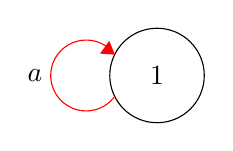
\begin{tikzpicture}[scale=0.2]
\tikzstyle{every node}+=[inner sep=0pt]
\draw [black] (38.6,-27.3) circle (3);
\draw (38.6,-27.3) node {$1$};
\draw [red] (35.92,-28.623) arc (324:36:2.25);
\draw (31.35,-27.3) node [left] {$a$};
\fill [red] (35.92,-25.98) -- (35.57,-25.1) -- (34.98,-25.91);
\end{tikzpicture}
\end{center}


Ahora, realizamos un proceso conocido como escaneo de relatores bajo las clases. Como cada relator $w$ representa la identidad cuando es visto como elemento  de $G$, se debe cumplir $\alpha^w = \alpha$, para toda clase $\alpha \in \Omega$ y toda palabra $w \in R$. En términos del grafo de Schreier, se debe poder realizar un recorrido (marcado por cada relator) partiendo y terminando en el mismo vértice.
Esto se cumple para $1^{a^3}=1$, pero no para el resto, por lo que el escaneo se interrumpe. Por esta razón, se deben realizar nuevas definiciones para que el proceso de escaneo se complete para todas las clases.

El siguiente relator que se debe escanear es $b^3$ sobre la clase $1$, que no se cumple. Como no se puede asegurar $1^b=1$, necesitamos definir nuevas clases. $1^b:=2$, $2^b:=3$ y $3^b:=1$.  Equivalentemente, estas definiciones equivalen a $1^{b^{-1}}=3$, $2^{b^{-1}}=1$ y $3^{b^{-1}}=2$. 



\begin{center}
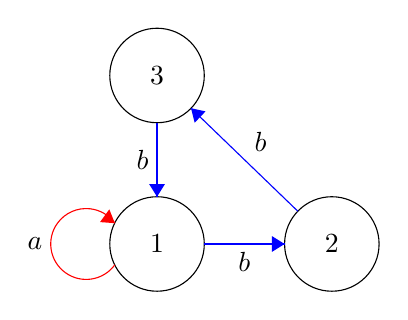
\begin{tikzpicture}[scale=0.2]
\tikzstyle{every node}+=[inner sep=0pt]
\draw [black] (36.2,-30.8) circle (3);
\draw (36.2,-30.8) node {$1$};
\draw [black] (47.3,-30.8) circle (3);
\draw (47.3,-30.8) node {$2$};
\draw [black] (36.2,-20.1) circle (3);
\draw (36.2,-20.1) node {$3$};
\draw [red] (33.52,-32.123) arc (324:36:2.25);
\draw (28.95,-30.8) node [left] {$a$};
\fill [red] (33.52,-29.48) -- (33.17,-28.6) -- (32.58,-29.41);
\draw [blue] (36.2,-23.1) -- (36.2,-27.8);
\fill [blue] (36.2,-27.8) -- (36.7,-27) -- (35.7,-27);
\draw (35.7,-25.45) node [left] {$b$};
\draw [blue] (45.14,-28.72) -- (38.36,-22.18);
\fill [blue] (38.36,-22.18) -- (38.59,-23.1) -- (39.28,-22.38);
\draw (42.77,-24.97) node [above] {$b$};
\draw [blue] (39.2,-30.8) -- (44.3,-30.8);
\fill [blue] (44.3,-30.8) -- (43.5,-30.3) -- (43.5,-31.3);
\draw (41.75,-31.3) node [below] {$b$};
\end{tikzpicture}
\end{center}


Como podemos comprobar, el vértice $1$ cumple $1^{a^3}=1$ y $1^{b^3}=1$; los vértices $2$ y $3$ cumplen $2^{b^3}=1$ y $3^{b^3}=1$, respectivamente, pero aún falta cumplir la relación $b^3$ sobre los vértices $2$ y $3$, y $aba^{-1}b^{-1}$ sobre todos los vértices. 

Para hacer cumplir $\alpha^{w}=\alpha$ para los vértices $2,3$ y todas las relaciones, se define $2^a:=2$ y $3^a:=3$. Estas dos definiciones bastan para terminar el escaneo en todos los vértices y todo relator ya que el tercer relator termina satisfaciéndose en todo vértice, obteniendo el siguiente grafo de Schreier:

\vspace{0.2cm}

\begin{center}
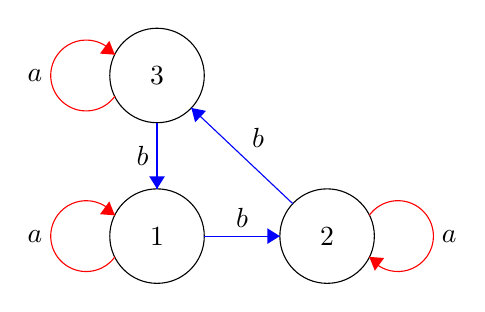
\begin{tikzpicture}[scale=0.2]
\tikzstyle{every node}+=[inner sep=0pt]
\draw [black] (25.7,-34) circle (3);
\draw (25.7,-34) node {$1$};
\draw [black] (36.5,-34) circle (3);
\draw (36.5,-34) node {$2$};
\draw [black] (25.7,-23.8) circle (3);
\draw (25.7,-23.8) node {$3$};
\draw [blue] (28.7,-34) -- (33.5,-34);
\fill [blue] (33.5,-34) -- (32.7,-33.5) -- (32.7,-34.5);
\draw (31.1,-33.5) node [above] {$b$};
\draw [blue] (34.32,-31.94) -- (27.88,-25.86);
\fill [blue] (27.88,-25.86) -- (28.12,-26.77) -- (28.81,-26.05);
\draw (32.12,-28.42) node [above] {$b$};
\draw [blue] (25.7,-26.8) -- (25.7,-31);
\fill [blue] (25.7,-31) -- (26.2,-30.2) -- (25.2,-30.2);
\draw (25.2,-28.9) node [left] {$b$};
\draw [red] (23.02,-35.323) arc (-36:-324:2.25);
\draw (18.45,-34) node [left] {$a$};
\fill [red] (23.02,-32.68) -- (22.67,-31.8) -- (22.08,-32.61);
\draw [red] (39.18,-32.677) arc (144:-144:2.25);
\draw (43.75,-34) node [right] {$a$};
\fill [red] (39.18,-35.32) -- (39.53,-36.2) -- (40.12,-35.39);
\draw [red] (23.02,-25.123) arc (-36:-324:2.25);
\draw (18.45,-23.8) node [left] {$a$};
\fill [red] (23.02,-22.48) -- (22.67,-21.6) -- (22.08,-22.41);
\end{tikzpicture}
\end{center}
El vértice $1$ equivale a la clase $H\tau(1)=H$, el vértice $2$ a la clase $H\tau(2)=Hb$ y, el $3$ a la clase $H\tau(3)=Hb^{-1}$.
Este grafo de Schreier es equivalente a la siguiente tabla de clases:


\begin{table}[H]
\centering
\begin{tabular}{c|cccc}
    & $a$ & $a^{-1}$ & $b$ & $b^{-1}$ \\
    \hline
$1$ & $1$ & $1$      & $2$ & $3$      \\
$2$ & $2$ & $2$      & $3$ & $1$      \\
$3$ & $3$ & $3$      & $1$ & $2$     
\end{tabular}
\end{table}



Como todas las clases se escanean correctamente bajo todos los relatores, y todas las entradas en la tabla de clases están definidas, el proceso termina, y el índice de $H$ en $G$, $[G:H]$, coincide con el número de clases o vértices definidos, que son $3$. 







\newpage
A continuación, enunciaremos unas \textbf{propiedades} que se deben cumplir, y en el Teorema \ref{important}, se probará que el algoritmo es correcto y que los generadores de Schreier dan lugar a una representación por permutaciones del grupo $G$.

    \begin{enumerate}
        \item $1 \in \Omega$ y $\tau(1)=\epsilon$ .
        \item $\alpha^x=\beta \Longleftrightarrow \beta^{x^{-1}}=\alpha$.
        \item Si $\alpha^x=\beta$, entonces $H\tau(\alpha)x=H\tau(\beta)$.
        \item Para todo $\alpha \in \Omega$, $1^{\tau(\alpha)}$ está definido y es igual a $\alpha$.
    \end{enumerate}

        \begin{theorem} \label{important}
        Supongamos que:
            
        \renewcommand{\theenumi}{}
        \begin{enumerate}[(i)]
            \item Las propiedades $1-4$ anteriores se cumplen. \label{uno}
            \item La tabla de clases está completa.
            \item $1$ escanea satisfactoriamente para todo $w\in Y$.
            \item Todo $\alpha \in \Omega$ se escanea correctamente para todo $w \in R$.
        \end{enumerate}
        Entonces, $[G:H] = |\Omega|$. Además, para cada $x \in A$, la aplicación:
        \begin{align*}
            \varphi(x) \colon \Omega &\to \Omega \\
            \alpha & \mapsto \alpha^x
        \end{align*}
        es una permutación de $\Omega$ y $\varphi$ extiende a un homomorfismo de $G=\langle X \mid R \rangle$ a $S(\Omega)$, que es equivalente a la acción de $G$ sobre las clases de $H$ por la multiplicación a la derecha.
        \end{theorem}
        
        \begin{proof}
        Por la propiedad $2$, $\varphi(x)$ y $\varphi(x^{-1})$ son aplicaciones inversas para cualquier $x\in A$ y entonces, $\varphi(x)$ es una permutación. La suposición (\RN{4}) dice que para cualquier $w=x_1 \ldots x_r \in R$, se tiene $\alpha^{\varphi(x_1) \varphi(x_2) \ldots \varphi(x_r)}=\alpha$, para todo $\alpha \in \Omega$. Así, $\varphi(x_1)\varphi(x_2)\cdots \varphi(x_r)=1_{S(\Omega)}$. Por lo que $\varphi$ extiende a un homomorfismo de grupos, que viene dado por $\varphi^* \colon \langle X \mid R \rangle \rightarrow S(\Omega)$ ; $\varphi^*(xN)=\varphi(x)$, para todo $x \in X $, donde $N=\operatorname{ker}(\varphi^*)$.
        
        Para probar la equivalencia de $\varphi$ con la acción de $G$ sobre el conjunto $C$ de clases de $H$, definimos:
        \begin{align*}
            \overline{\tau} \colon \Omega & \to C \\
            \overline{\tau}(\alpha) & = H \tau(\alpha) 
        \end{align*}
        Para cualquier $v \in A^*$, la suposición (\RN{2}) y la propiedad $3$ implican que $\overline{\tau}(1^v)=Hv$, por lo que $\overline{\tau}$ es sobreyectiva. Si  $\overline{\tau}(\alpha)= \overline{\tau}(\beta)$, entonces $H\tau(\alpha)=H\tau(\beta)$, por lo que $\tau(\alpha)\tau(\beta)^{-1} \in H$. Así, $\tau(\alpha)\tau(\beta)^{-1}$ es el producto $w_1\cdots w_r$, donde $w_i \in Y\cup Y^{-1}$. \\
        Por la hipótesis  (\RN{3}), se tiene $1^{w_i}=1$ para todo $w_i$. Así, $1^{\tau(\alpha)\tau(\beta)^{-1}}=1$, y por la propiedad $4$, $\alpha=1^{\tau(\alpha)}=1^{\tau(\beta)}=\beta$. Se tiene que $\overline{\tau}$ es inyectiva, y por tanto, biyectiva, luego $[G:H]=|\Omega|$ y, por la propiedad $3$, $\overline{\tau}$ define una equivalencia entre $\varphi$ y la acción de $G$ sobre $C$ por la multiplicación a la derecha.
        \end{proof}






\newpage
\subsubsection{Proceso definición de clases} 

Si $\alpha^x$ no está definido para algún $\alpha \in [1,\ldots,n]$, $x\in A$, la manera más simple es añadir un nuevo elemento $\beta$ a $\Omega$ y definir $\alpha^x:= \beta$. Esto es lo que se conoce como \textit{definición de una clase} y el pseudocódigo es el que se muestra a continuación: 

\begin{center}
\begin{minipage}{.65\linewidth}
    \begin{algorithm}[H] 
    \SetAlgoLined
    	\caption{Define}
    	\KwData{ $\alpha \in \Omega$ , $x \in A$ , $\alpha^x$ undefined }
    	\KwResult{ $C$: Coset Table with new $\alpha^x$ definition}

            \If{n  = M}{
                \textbf{abort} \\
            }
            $n := n+1$, $\quad \beta := n$, $\quad p(\beta):=\beta$ \\
    	    $\alpha^x := \beta$ , $\quad \beta^{x^{-1}} := \alpha$ 
    
    \end{algorithm} 
\end{minipage}
\end{center}

\vspace{0.5cm}
Como podemos observar, el proceso previo al de la definición de la clase, es el de comprobar si hay espacio disponible, es decir, $n$ debe ser menor que $M$.
Además, cuando se llama al procedimiento \textit{Define} anterior para definir $\alpha^x:= \beta$, también se debe definir $\beta^{x^{-1}}:=\alpha$ por la propiedad $2$ anterior.


Como consecuencia del proceso de definición de una clase, se han programado los siguientes métodos:
\begin{itemize}
    \item \textit{isAlived($\alpha$)}: comprueba que la clase pasada por argumento está viva, es decir, pertenece a $\Omega$.
    \item \textit{Undefine($\alpha, x$)}: se trata de la operación opuesta a \texttt{define} y su función será la de eliminar el valor $\alpha^x$ para un $\alpha \in \Omega$ y $x \in A$ de la tabla $C$.
    
    \item \textit{isDefined($\alpha, x$)}: se encarga de comprobar si el valor $\alpha^x$ para un $\alpha \in \Omega$ y $x \in A$ está definido, devolviendo $True$ en caso afirmativo.
\end{itemize}







\subsubsection{Coincidencias} \label{siguiente}

\iffalse
\begin{definition}
    Dadas $\alpha, \beta \in \Omega$ dos clases, se dice que existe una \textit{coincidencia} cuando para algún $i$ con $i\leq i \leq r+1$, se tiene $w=st$ con $s=x_1x_2\cdots x_{i-1}$ , $t=x_ix_{i+1}\cdots x_r$  y $\alpha:=\gamma^s$ y $\beta:=\gamma^{t-1}$.
\end{definition}
\fi

%Véase la Sección \ref{ident} para un ejemplo práctico.



En nuestro algoritmo, para almacenar la relación de equivalencia de una clase se ha programado la clase \textit{EquivalenceClass}. En ella, se lleva un registro de las relaciones de equivalencia, donde cada una estará representada por su menor elemento. Destacamos los siguientes métodos:
\begin{itemize}
    \item \textit{rep(k)}: devuelve el menor elemento (su representante) de la clase de equivalencia de la clase $k$. Este método hace uso de la aplicación $p: [1,\ldots,n] \to [1,\ldots,n]$ descrita anteriormente.
    \item \textit{merge(k,$\lambda$)}: se opera sobre las dos clases de equivalencia pasadas por argumento, devolviendo su representante o $-1$ si las dos clases son iguales.
\end{itemize}


Como ya hemos comentado, una coincidencia ocurre cuando dos clases distintas $\alpha$ y $\beta$ con $\alpha < \beta$ representan la misma clase, es decir, tienen el mismo representante.
Se debe registrar esta ocurrencia llamando al método $merge(\alpha, \beta$) anterior, el cual fija $p(\beta)=\alpha$, para indicar que $\beta$ es equivalente a $\alpha$, e introducir $\beta$ en una cola (queue) de clases que deben ser procesadas.  $p(\alpha)=\alpha$ se debe  mantener  ya que $\alpha$ es el representante de ambas clases y debe perdurar en $\Omega$. 



El pseudocódigo asociado a este método es el siguiente:






\begin{center}
\begin{minipage}{.7\linewidth}
    \begin{algorithm}[H] 
    \SetAlgoLined
    	\caption{Coincidence}
    	\KwData{ $\alpha, \beta \in \Omega$ }

    	    $merge$($\alpha, \beta$) \\
    	    \While{$|queue|>0$}{
    	        
    	        $y := queue.front()$, $\quad$ $queue.pop()$ \\
    	        
    	        \For{$x \in A$}{
    	        
    	            \If{$y^x$ isDefined}{
    	                $\rho = rep(y^x)$ \\
    	            
        	            $undefine$  $\rho^{x^{-1}}$\\
        	            $\mu := rep(y)$, $\quad \sigma := rep(\rho)$ \\ 
        	            \vspace{0.2cm}
        	            \uIf{$\mu^x$ isDefined}{
        	                \vspace{0.1cm}
        	                $merge$($\sigma, \mu^x$) \\
        	            }
        	            
        	            \uElseIf{$\sigma^{x^{-1}}$ isDefined}{
        	                $merge$($\mu, \sigma^{x^{-1}}$)
        	           }
        	           
        	            \Else{
        	                $\mu^x := \sigma$ , $ \quad \sigma^{x^{-1}} := \mu$
        	           }
    	           }
    	        }
    	    }
    	
    \end{algorithm} 
\end{minipage}
\end{center}

Sea $y$ un elemento de la cola que debe ser procesado. Toda la información de la clase $y$ debe ser transferida a la clase $rep(y)$ ya que va a ser borrada. Para cada elemento $x \in A$, se debe comprobar si $y^x$ está definido, supongamos que $y^x=\rho$. Entonces, lo primero se debe llevar a cabo es borrar esta entrada ya que no queremos que $y$ permanezca en la fila $\rho$. De este modo, queda eliminada la clase $y$ de la tabla. En términos del grafo de Schreier, se han borrado todas las aristas que llegan al vértice $y$. Sin embargo, debemos completar el grafo con nuevas aristas que entran y salen de su representante $rep(y)$.


Consideramos $\overline{y}=rep(y)$ y $\overline{\rho}=rep(\rho)$. Distingamos los siguientes casos:
\begin{enumerate}
    \item  Si se tiene una entrada definida $\overline{y}^x$, que es igual a $w$, entonces llamamos a $merge(\overline{\rho}, w)$. 
\item Si se tiene una entrada definida $\overline{\rho}^{x^{-1}}=w$, entonces realizamos un $merge(\overline{y}, w)$. 
\item En caso contrario, se tendrán que definir las entradas $\overline{y}^x:=\overline{\rho}$ y $\overline{\rho}^{x^{-1}}:=\overline{y}$.
\end{enumerate}



\newpage
\subsubsection{Escaneo}
Sigamos ahora con el \textit{proceso de escaneo}. Este procedimiento recibe una clase $\alpha \in \Omega$ y una palabra $w \in A$ y se encarga de comprobar si la palabra $w$ se satisface para la clase $\alpha$, es decir, $\alpha^w=\alpha$. En otras palabras, si partiendo desde el vértice $\alpha$ se puede realizar un recorrido marcado por $w$ que acabe en el mismo vértice.

El método encargado de comprobar lo anterior se denomina \textit{ScanAndFill} y el pseudocódigo asociado es el siguiente:




\begin{center}
\begin{minipage}{.6\linewidth}
    \begin{algorithm}[H] 
    \SetAlgoLined
    
    	\caption{ScanAndFill}
    	\KwData{ $ \alpha \in \Omega$, $w = x_1,\ldots, x_r$ with $x_i \in A$ }

    	    $i, j := 0, r$ , $\quad f, b := \alpha, \alpha$  \\
            
            \While{True}{
                \textcolor{blue}{*Scan forward*} \\
                \While{$i \leq j$ and $f^{x_i}$ isDefined }{
                    $f := f^{x_i}$ , $ \quad i := i+1$
                }

                \If{$i>j$}{ 

                    \If{ $f \not = b$}{
                        $Coincidence$($f,b$)
                    }
                    \textbf{return}

                }
                \textcolor{blue}{*Scan backwards*} \\
                \While{$j \geq i$ and $b^{x_i^{-1}}$ isDefined}{
                    $b := b^{x_i^{-1}}$, $\quad j:=j-1$
                }
            
                \uIf{$j<i$}{
                    $Coincidence$($f,b$) \\
                    \textbf{return} \\
                    \vspace{0.3cm}

                }
                
                \uElseIf{$j=i$}{
                    $f^{x_i} :=  b$ , $\quad b^{x_i^{-1}} := f$ \\
                    \textbf{return}
                    
                }  
                \Else{
                    $define$($f, x_i$)
                }
            } 
        
    \end{algorithm} 
\end{minipage}
\end{center}

En método se ejecuta ininterrumpidamente hasta que la fila de la clase $\alpha \in \Omega$ se rellene por completo. Se puede realizar el proceso de escaneo hacia adelante o hacia atrás, al igual que se hizo en la Sección \ref{TC} con las tablas de relatores.
Cuando el escaneo es satisfactorio salimos del método con una llamada a return. Antes de esta llamada pueden ocurrir dos situaciones, que se detecte una deducción o una coincidencia entre dos clases. En este último caso,  se debe llamar al método $Coincidence$ para procesarlas.
Por último, cuando el método no es capaz de escanear la palabra $w$ sobre la clase $\alpha$ de forma satisfactoria, se debe definir una nueva clase y seguir hasta que así lo sea.






\subsubsection{Método principal}


Explicaremos a continuación la idea que sigue el método  \textit{HLT}:
\begin{enumerate}
    \item En primer lugar, se inicializa una tabla de clases $C$ vacía para el grupo $G$ dado por generadores $X$ y relatores $R$.
    \item Para cada uno de los generadores de $H$, se llama al método \textit{ScanAndFill} para realizar un escaneo completo sobre la primera clase $1$.
    

    
    \item Se recorre el conjunto de clases vivas $\Omega$ y relatores de $G$, comprobando que cada clase de $\Omega$ se escanee por completo siguiendo cada  $w \in R$, es decir, $\alpha^w=\alpha$ para todo $\alpha \in \Omega$, $w\in R$. Si no es así, se realizarán sucesivas definiciones para que el escaneo se complete o se alcance la cota $M$ establecida.

\end{enumerate}


El pseudocódigo asociado al método principal \textit{HLT} es el siguiente:
\begin{center}
\begin{minipage}{.7\linewidth}
    \begin{algorithm}[H] 
    \SetAlgoLined
    	\caption{CosetEnumeration}
    	\KwData{ $G = \langle X \mid R\rangle$  : group, $H=\langle Y \rangle $ : subgroup.}
    	\KwResult{ $C$: Coset Table for $G/H$.}
            
            Initialize an empty Coset table for $\langle X\mid R \rangle$. \\
    	    
    	    \For{$w \in Y$ }{
    	        $ScanAndFill$($1, w$) \\
    	    }
    	    
    		\For{$\alpha \in \Omega$}{
    		    \For{$w \in R$}{
    		        %\If{not isAlive($\alpha$)}{
    		        %
    		        %    \textbf{continue} \\
    		        %}
    		        %$ScanAndFill$($\alpha,w$) \\
    		        
    		        \If{isAlive($\alpha$)}{
    		            $ScanAndFill$($\alpha,w$) \\
    		        }
    		    }
    		    \If{isAlive($\alpha$)}{
    		        \For{$x \in A$}{
    		            \If{not isDefined($\alpha$,x)}{
    		                $define$($\alpha,x$)\\
    		            }
    		        }
    		    }
    		}
    	
    \end{algorithm} 
\end{minipage}
\end{center}



Hay que tener cuidado con el bucle que opera sobre las clases de $\Omega$ ya que este conjunto no está fijo, es decir,  inicialmente contiene la clase $1$ pero se van añadiendo nuevas cada vez que sea necesario. 

Como hemos comentado anteriormente, uno de los problemas del \textit{Algoritmo de Todd Coxeter} es el gran uso de memoria que requiere. El método descrito anteriormente no es siempre óptimo en términos del máximo valor $max{|\Omega|}$ escogido, pero en la mayoría de las veces cumple su función correctamente, proporcionando así suficiente memoria para que el algoritmo termine.
 En nuestra implementación, el valor $M=max|\Omega| = 1E6$ se ha elegido tras varias ejecuciones en diferentes ejemplos de grupos, por lo que en principio, el espacio no será un problema.



\subsection{Funcionalidades y uso} \label{fyu}
El \textit{Algoritmo de Todd Coxeter} se ha programado en \textit{ToddCoxeter.py}. Destacamos los siguientes métodos implementados:
    \begin{itemize}
        \item \textit{readGroup}: implementación de una función que nos ayudará a leer los grupos por ficheros. Por orden, se leerán los generadores del grupo $G$, sus relaciones y los generadores del subgrupo $H$. En el directorio /Group se proporcionaran ejemplos de diferentes grupos, tanto de aquellos con los que se han trabajado como los que no.
        
        \item \textit{CosetEnumeration}: método principal para llamar al algoritmo y generar la tabla de clases laterales de $G/H$.
        
        \item \textit{coset\_table} , \textit{schreier\_graph}: el primer método devuelve la tabla de clases laterales de $G/H$, donde el número de filas coincide con el índice $[G:H]$ (sin contar la cabecera). El segundo método calcula el grafo de Schreier resultante, que es equivalente a la tabla de clases anterior.  
        
        Sean $w_1, w_2$  dos palabras dadas como producto de generadores. Se puede comprobar de forma sencilla si representan el mismo elemento. Para ello, se debe partir del vértice $1$, seguir el recorrido de la palabra en el grafo y ver si acaban en el mismo vértice. Por esta razón, el \textit{Algoritmo de Todd Coxeter} es un algoritmo que resuelve el Problema de Palabras.
        
                
        \item \textit{usedCosets}, \textit{FinalCosets}: el primer método devuelve el número de clases usadas durante la ejecución del algoritmo mientras el segundo devuelve el número de clases vivas, que coincidirán con el índice de $[G:H]$ si el algoritmo termina. Si $H$ es el subgrupo trivial entonces este método devuelve el orden de $G$.
        
        
        \item \textit{getGenerators}: como se ha visto en el Teorema \ref{important}, se puede obtener una representación por permutaciones del grupo $G$. Esta función se encarga de obtener los generadores de Schreier, que más adelante pueden ser usados en el constructor de la clase Group para definir el grupo que generan.
        
        

    \end{itemize}
    





    


%En primer lugar, se realizará una explicación guiada del procedimiento mediante, dejando %la ejecución de diferentes ejemplos en la siguiente sección. En esta sección se verán %diferentes ejemplos de ejecuciones del algoritmo de Todd Coxeter bajo el siguiente %escenario.

%Sea $G$ un grupo definido por una presentación $G = \langle X \mid R \rangle $, donde $X$ es el conjunto de generadores y $R$ el conjunto de relatores. Sea $H = \langle h_1, h_2, \ldots , h_r \rangle \leq G$ un subgrupo. 

%\begin{remark}
%En la mayoría de los ejemplos consideraremos $H=\{1\}$ ya que así la tabla de clases %refleja la acción del grupo $G$. No obstante, trataremos ejemplos en los que el subgrupo %$H$ no sea el trivial.
%\end{remark}


    

En primer lugar, importamos las librerías que se utilizarán:
\begin{itemize}
    \item  \texttt{Group}: fichero principal de la librería. En él se encuentran las principales clases y funciones para definir los diferentes grupos y sirve para identificar y dar estructura de grupo al conjunto de generadores y relatores dados como entrada. 
    \item  \texttt{ToddCoxeter}: contiene la implementación del \textit{Algoritmo de Todd Coxeter} junto a todas las funcionalidades descritas anteriormente. 


    \begin{tcolorbox}[breakable, size=fbox, boxrule=1pt, pad at break*=1mm,colback=cellbackground, colframe=cellborder]
%\prompt{In}{incolor}{1}{\boxspacing}
\begin{Verbatim}[commandchars=\\\{\}]
\PY{k+kn}{from} \PY{n+nn}{Group} \PY{k+kn}{import} \PY{o}{*}
\PY{k+kn}{from} \PY{n+nn}{ToddCoxeter} \PY{k+kn}{import} \PY{n}{CosetTable}\PY{p}{,} \PY{n}{readGroup}
\end{Verbatim}
\end{tcolorbox}

\end{itemize}



El procedimiento a seguir se desarrollará a continuación y se ilustrará con el siguiente ejemplo sencillo:
\[
G=\langle a,b \mid a^2, b^2, ab=ba \rangle \quad y \quad H=\{1\}.
\]

\begin{enumerate}
\item Leemos los datos de entrada, ya sea mediante variables para definir el grupo o
  haciendo uso del método \textit{readGroup}, en el que se le ha de especificar la ruta del fichero donde está el grupo.
  
  \begin{tcolorbox}[breakable, size=fbox, boxrule=1pt, pad at break*=1mm,colback=cellbackground, colframe=cellborder]
\prompt{In}{incolor}{1}{\boxspacing}
\begin{Verbatim}[commandchars=\\\{\}]
\PY{n}{gen} \PY{o}{=} \PY{p}{[}\PY{l+s+s1}{\PYZsq{}}\PY{l+s+s1}{a}\PY{l+s+s1}{\PYZsq{}}\PY{p}{,}\PY{l+s+s1}{\PYZsq{}}\PY{l+s+s1}{b}\PY{l+s+s1}{\PYZsq{}}\PY{p}{]}
\PY{n}{rels} \PY{o}{=} \PY{p}{[}\PY{l+s+s1}{\PYZsq{}}\PY{l+s+s1}{aa}\PY{l+s+s1}{\PYZsq{}}\PY{p}{,}\PY{l+s+s1}{\PYZsq{}}\PY{l+s+s1}{bb}\PY{l+s+s1}{\PYZsq{}}\PY{p}{,}\PY{l+s+s1}{\PYZsq{}}\PY{l+s+s1}{abAB}\PY{l+s+s1}{\PYZsq{}}\PY{p}{]}
\PY{n}{genH} \PY{o}{=} \PY{p}{[}\PY{p}{]}
\end{Verbatim}
\end{tcolorbox}
  
  
  
\item Creamos un objeto de la clase \textit{CosetTable}. Después, llamamos al método \textit{CosetEnumeration} para aplicar el \textit{Algoritmo de Todd Coxeter}.

\begin{tcolorbox}[breakable, size=fbox, boxrule=1pt, pad at break*=1mm,colback=cellbackground, colframe=cellborder]
\prompt{In}{incolor}{2}{\boxspacing}
\begin{Verbatim}[commandchars=\\\{\}]
\PY{n}{G} \PY{o}{=} \PY{n}{CosetTable}\PY{p}{(}\PY{n}{gen}\PY{p}{,}\PY{n}{rels}\PY{p}{,} \PY{n}{genH}\PY{p}{)}
\PY{n}{G}\PY{o}{.}\PY{n}{CosetEnumeration}\PY{p}{(}\PY{p}{)}
\end{Verbatim}
\end{tcolorbox}


  
Podemos mostrar la tabla de clases laterales de $G/H$, que se obtiene mediante el método \textit{coset\_table}.

    \begin{tcolorbox}[breakable, size=fbox, boxrule=1pt, pad at break*=1mm,colback=cellbackground, colframe=cellborder]
\prompt{In}{incolor}{3}{\boxspacing}
\begin{Verbatim}[commandchars=\\\{\}]
\PY{n}{T} \PY{o}{=} \PY{n}{G}\PY{o}{.}\PY{n}{coset\PYZus{}table}\PY{p}{(}\PY{p}{)}
\PY{n+nb}{print}\PY{p}{(}\PY{n}{T}\PY{p}{)}
\end{Verbatim}
\end{tcolorbox}

    \begin{center}
    \adjustimage{max size={0.29\linewidth}{0.29\paperheight}}{img/1g.png}
    \end{center}


Como hemos comentado anteriormente, el número de filas sin contar las cabeceras indica el número de elementos del grupo $G/H$, que coincide con el índice $[G:H]$. En este ejemplo, se tiene:
\[
    [G:H] = \frac{|G|}{|H|} = \frac{|G|}{1} = |G| = 4 \: .
\]

\newpage
Equivalentemente, el grafo de Schreier asociado se llama de la siguiente forma:

    \begin{tcolorbox}[breakable, size=fbox, boxrule=1pt, pad at break*=1mm,colback=cellbackground, colframe=cellborder]
\prompt{In}{incolor}{4}{\boxspacing}
\begin{Verbatim}[commandchars=\\\{\}]
\PY{n}{G}\PY{o}{.}\PY{n}{schreier\PYZus{}graph}\PY{p}{(}\PY{n}{notes}\PY{o}{=}\PY{k+kc}{False}\PY{p}{)}
\end{Verbatim}
\end{tcolorbox}

    \begin{center}
    \adjustimage{max size={0.4\linewidth}{0.26\paperheight}}{img/code_7_0.png}
    \end{center}



\item El siguiente paso es el de obtener los generadores de Schreier y definir el grupo como aquel generado por estos elementos.
  
    \begin{tcolorbox}[breakable, size=fbox, boxrule=1pt, pad at break*=1mm,colback=cellbackground, colframe=cellborder]
\prompt{In}{incolor}{5}{\boxspacing}
\begin{Verbatim}[commandchars=\\\{\}]
\PY{k}{def} \PY{n+nf}{print\PYZus{}gens}\PY{p}{(}\PY{n}{gens}\PY{p}{)}\PY{p}{:}
    \PY{k}{for} \PY{n}{i} \PY{o+ow}{in} \PY{n+nb}{range}\PY{p}{(}\PY{n+nb}{len}\PY{p}{(}\PY{n}{gens}\PY{p}{)}\PY{p}{)}\PY{p}{:}
        \PY{n+nb}{print}\PY{p}{(}\PY{l+s+sa}{f}\PY{l+s+s2}{\PYZdq{}}\PY{l+s+s2}{g}\PY{l+s+si}{\PYZob{}}\PY{n}{i}\PY{l+s+si}{\PYZcb{}}\PY{l+s+s2}{ = }\PY{l+s+si}{\PYZob{}}\PY{n}{gens}\PY{p}{[}\PY{n}{i}\PY{p}{]}\PY{l+s+si}{\PYZcb{}}\PY{l+s+s2}{\PYZdq{}}\PY{p}{)}
        
\PY{n}{generators} \PY{o}{=} \PY{n}{G}\PY{o}{.}\PY{n}{getGenerators}\PY{p}{(}\PY{p}{)}
\PY{n}{print\PYZus{}gens}\PY{p}{(}\PY{n}{generators}\PY{p}{)}
\end{Verbatim}
\end{tcolorbox}  

 \begin{tcolorbox}[breakable, size=fbox, boxrule=.5pt, pad at break*=1mm, opacityfill=0]
\prompt{Out}{outcolor}{5}{\boxspacing}
    \begin{Verbatim}[commandchars=\\\{\}]
g0 = (1, 2)(3, 4)
g1 = (1, 3)(2, 4)
    \end{Verbatim}
\end{tcolorbox}
    

En este momento, tenemos los generadores que definen al grupo. En particular, en este ejemplo el grupo estará definido por
$G = \langle \, g0, \, g1 \, \rangle $.


\begin{tcolorbox}[breakable, size=fbox, boxrule=1pt, pad at break*=1mm,colback=cellbackground, colframe=cellborder]
\prompt{In}{incolor}{6}{\boxspacing}
\begin{Verbatim}[commandchars=\\\{\}]
\PY{n}{Gr} \PY{o}{=} \PY{n}{Group(elems=generators)}
\end{Verbatim}
\end{tcolorbox}  
 
 
\item  Usar el método \textit{is\_isomorphic} para identificar cada grupo con
  grupos conocidos.
  
  
Observando la presentación dada, no es dificil ver que el grupo debe ser isomorfo al Grupo de Klein:

\begin{tcolorbox}[breakable, size=fbox, boxrule=1pt, pad at break*=1mm,colback=cellbackground, colframe=cellborder]
\prompt{In}{incolor}{7}{\boxspacing}
\begin{Verbatim}[commandchars=\\\{\}]
\PY{n}{K} \PY{o}{=} \PY{n}{KleinGroup}\PY{p}{(}\PY{p}{)}
\PY{n}{Gr}\PY{o}{.}\PY{n}{is\PYZus{}isomorphic}\PY{p}{(}\PY{n}{K}\PY{p}{)}
\end{Verbatim}
\end{tcolorbox}

\begin{tcolorbox}[breakable, size=fbox, boxrule=.5pt, pad at break*=1mm, opacityfill=0]
\prompt{Out}{outcolor}{7}{\boxspacing}
\begin{Verbatim}[commandchars=\\\{\}]
True
\end{Verbatim}
\end{tcolorbox}
  
  
\end{enumerate}

 
\newpage
\subsection{Ejemplos}

En la siguiente sección se estudiarán diferentes ejemplos de grupos finitamente presentados. El objetivo es identificar la presentación dada estableciendo isomorfismos con grupos estudiados.

Consideramos el siguiente grupo, que se encuentra en \textit{Groups/1.txt}.
\begin{align*} \label{1st}
    G = \langle a,b\; | \; ab^{-1}b^{-1}a^{-1}bbb, b^{-1}a^{-1}a^{-1}baaa\rangle \quad y \quad H = \{ 1\}.
\end{align*}

\begin{enumerate}
En primer lugar, usamos el método \textit{readGroup} para leerlo:


    \begin{tcolorbox}[breakable, size=fbox, boxrule=1pt, pad at break*=1mm,colback=cellbackground, colframe=cellborder]
\prompt{In}{incolor}{1}{\boxspacing}
\begin{Verbatim}[commandchars=\\\{\}]
\PY{n}{file} \PY{o}{=} \PY{l+s+s2}{\PYZdq{}}\PY{l+s+s2}{Groups/1.txt}\PY{l+s+s2}{\PYZdq{}}
\PY{n}{f} \PY{o}{=} \PY{n}{readGroup}\PY{p}{(}\PY{n}{file}\PY{p}{)}
\PY{n+nb}{print}\PY{p}{(}\PY{n}{f}\PY{p}{)}
\end{Verbatim}
\end{tcolorbox}

    \begin{Verbatim}[commandchars=\\\{\}]
(['a', 'b'], ['aBBAbbb', 'BAAbaaa'], [])
    \end{Verbatim}

De igual modo que en el ejemplo anterior, aplicamos el \textit{Algoritmo de Todd Coxeter}. 

\begin{tcolorbox}[breakable, size=fbox, boxrule=1pt, pad at break*=1mm,colback=cellbackground, colframe=cellborder]
\prompt{In}{incolor}{2}{\boxspacing}
\begin{Verbatim}[commandchars=\\\{\}]
\PY{n}{G} \PY{o}{=} \PY{n}{CosetTable}\PY{p}{(}\PY{n}{file}\PY{p}{)}
\PY{n}{G}\PY{o}{.}\PY{n}{CosetEnumeration}\PY{p}{(}\PY{p}{)}
\end{Verbatim}
\end{tcolorbox}




A continuación, mostramos la tabla de clases de $G/H$:

    \begin{tcolorbox}[breakable, size=fbox, boxrule=1pt, pad at break*=1mm,colback=cellbackground, colframe=cellborder]
\prompt{In}{incolor}{3}{\boxspacing}
\begin{Verbatim}[commandchars=\\\{\}]
\PY{n+nb}{print}\PY{p}{(}\PY{n}{G}\PY{o}{.}\PY{n}{table}\PY{p}{)}
\end{Verbatim}
\end{tcolorbox}

    \begin{center}
    \adjustimage{max size={0.28\linewidth}{0.28\paperheight}}{img/2g.png}
    \end{center}

Como vemos, únicamente hay una fila de clases, por lo que $[G:H]=1$ y, como $H=\{1\}$, $G$ debe ser necesariamente el grupo trivial. Como consecuencia, el grafo de Schreier posee un único vértice.
En este ejemplo, no es de utilidad darle estructura de grupo a $G$, en cambio, servirá para mostrar un ejemplo de un grupo sencillo en el que el número de clases que se usan es muy elevado. 

    \begin{tcolorbox}[breakable, size=fbox, boxrule=1pt, pad at break*=1mm,colback=cellbackground, colframe=cellborder]
\prompt{In}{incolor}{4}{\boxspacing}
\begin{Verbatim}[commandchars=\\\{\}]
\PY{n}{u} \PY{o}{=} \PY{n}{G}\PY{o}{.}\PY{n}{usedCosets}\PY{p}{(}\PY{p}{)}
\PY{n}{f} \PY{o}{=} \PY{n}{G}\PY{o}{.}\PY{n}{finalCosets}\PY{p}{(}\PY{p}{)}

\PY{n+nb}{print}\PY{p}{(}\PY{l+s+s2}{\PYZdq{}}\PY{l+s+s2}{Clases usadas: }\PY{l+s+si}{\PYZob{}\PYZcb{}}\PY{l+s+s2}{ }\PY{l+s+se}{\PYZbs{}n}\PY{l+s+s2}{ Clases vivas: }\PY{l+s+si}{\PYZob{}\PYZcb{}}\PY{l+s+s2}{\PYZdq{}}\PY{o}{.}\PY{n}{format}\PY{p}{(}\PY{n}{u}\PY{p}{,}\PY{n}{f}\PY{p}{)}\PY{p}{)}
\end{Verbatim}
\end{tcolorbox}


\begin{tcolorbox}[breakable, size=fbox, boxrule=.5pt, pad at break*=1mm, opacityfill=0]
\prompt{Out}{outcolor}{8}{\boxspacing}
    \begin{Verbatim}[commandchars=\\\{\}]
Clases usadas: 85
Clases vivas: 1
\end{Verbatim}
\end{tcolorbox}


\newpage
El siguiente grupo $G$ se encuentra definido en \textit{Groups/S3\_2.txt}, y como subgrupo $H\leq G$, tomamos aquel generado por $a$.
\begin{align*}
    G = \langle a,b \; | \; a^2 = b^2 = 1, (ab)^3=1\rangle \quad y \quad H= \langle a \rangle.
\end{align*}



    \begin{tcolorbox}[breakable, size=fbox, boxrule=1pt, pad at break*=1mm,colback=cellbackground, colframe=cellborder]
\prompt{In}{incolor}{1}{\boxspacing}
\begin{Verbatim}[commandchars=\\\{\}]
\PY{n}{file} \PY{o}{=} \PY{l+s+s2}{\PYZdq{}}\PY{l+s+s2}{Groups/S3\PYZus{}2.txt}\PY{l+s+s2}{\PYZdq{}}
\PY{n}{f} \PY{o}{=} \PY{n}{readGroup}\PY{p}{(}\PY{n}{file}\PY{p}{)}
\PY{n}{f}
\end{Verbatim}
\end{tcolorbox}

            \begin{tcolorbox}[breakable, size=fbox, boxrule=.5pt, pad at break*=1mm, opacityfill=0]
\prompt{Out}{outcolor}{2}{\boxspacing}
\begin{Verbatim}[commandchars=\\\{\}]
(['a', 'b'], ['aa', 'bb', 'ababab'], ['a'])
\end{Verbatim}
\end{tcolorbox}
        
Mostramos la tabla de clases de $G/H$ resultante tras aplicar el algoritmo.
    \begin{tcolorbox}[breakable, size=fbox, boxrule=1pt, pad at break*=1mm,colback=cellbackground, colframe=cellborder]
\prompt{In}{incolor}{3}{\boxspacing}
\begin{Verbatim}[commandchars=\\\{\}]
\PY{n+nb}{print}\PY{p}{(}\PY{n}{G}\PY{o}{.}\PY{n}{coset\PYZus{}table}\PY{p}{(}\PY{p}{)}\PY{p}{)}
\end{Verbatim}
\end{tcolorbox}

    \begin{center}
    \adjustimage{max size={0.28\linewidth}{0.28\paperheight}}{img/4g.png}
    \end{center}



Ahora, el grafo de Schreier equivalente:
    \begin{tcolorbox}[breakable, size=fbox, boxrule=1pt, pad at break*=1mm,colback=cellbackground, colframe=cellborder]
\prompt{In}{incolor}{4}{\boxspacing}
\begin{Verbatim}[commandchars=\\\{\}]
\PY{n}{G}\PY{o}{.}\PY{n}{schreier\PYZus{}graph}\PY{p}{(}\PY{n}{notes}\PY{o}{=}\PY{k+kc}{False}\PY{p}{)}
\end{Verbatim}
\end{tcolorbox}


    \begin{center}
    \adjustimage{max size={0.2\linewidth}{0.2\paperheight}}{img/code_48_0.png}
    \end{center}

Obtenemos los generadores de Schreier que definen al grupo, que se usarán, por el Teorema \ref{important}, para darle estructura de grupo de Permutaciones.

    \begin{tcolorbox}[breakable, size=fbox, boxrule=1pt, pad at break*=1mm,colback=cellbackground, colframe=cellborder]
\prompt{In}{incolor}{5}{\boxspacing}
\begin{Verbatim}[commandchars=\\\{\}]
\PY{n}{generators} \PY{o}{=} \PY{n}{G}\PY{o}{.}\PY{n}{getGenerators}\PY{p}{(}\PY{p}{)}
\PY{n}{print\PYZus{}gens}\PY{p}{(}\PY{n}{generators}\PY{p}{)}

\PY{n}{S} \PY{o}{=} \PY{n}{Group}\PY{p}{(}\PY{n}{elems}\PY{o}{=}\PY{n}{generators}\PY{p}{)}
\end{Verbatim}
\end{tcolorbox}


\begin{tcolorbox}[breakable, size=fbox, boxrule=.5pt, pad at break*=1mm, opacityfill=0]
\prompt{Out}{outcolor}{5}{\boxspacing}
    \begin{Verbatim}[commandchars=\\\{\}]
g0 = (2, 3)
g1 = (1, 2)
    \end{Verbatim}
\end{tcolorbox}

Vemos que el grupo es isomorfo a $S_3$, el grupo Simétrico de orden $6$.

    \begin{tcolorbox}[breakable, size=fbox, boxrule=1pt, pad at break*=1mm,colback=cellbackground, colframe=cellborder]
\prompt{In}{incolor}{6}{\boxspacing}
\begin{Verbatim}[commandchars=\\\{\}]
\PY{n}{S3} \PY{o}{=} \PY{n}{SymmetricGroup}\PY{p}{(}\PY{l+m+mi}{3}\PY{p}{)}
\PY{n}{S3}\PY{o}{.}\PY{n}{is\PYZus{}isomorphic}\PY{p}{(}\PY{n}{S}\PY{p}{)}
\end{Verbatim}
\end{tcolorbox}

            \begin{tcolorbox}[breakable, size=fbox, boxrule=.5pt, pad at break*=1mm, opacityfill=0]
\prompt{Out}{outcolor}{6}{\boxspacing}
\begin{Verbatim}[commandchars=\\\{\}]
True
\end{Verbatim}
\end{tcolorbox}
        

Otra forma equivalente para construir el grupo $S_3$ es mediante el producto
semidirecto $A_3 \rtimes K$, donde $K = \{1,(12)\}$. Véase el Ejemplo \ref{SnAn}.

    \begin{tcolorbox}[breakable, size=fbox, boxrule=1pt, pad at break*=1mm,colback=cellbackground, colframe=cellborder]
\prompt{In}{incolor}{7}{\boxspacing}
\begin{Verbatim}[commandchars=\\\{\}]
\PY{n}{A} \PY{o}{=} \PY{n}{AlternatingGroup}\PY{p}{(}\PY{l+m+mi}{3}\PY{p}{)}
\PY{n}{B} \PY{o}{=} \PY{n}{SymmetricGroup}\PY{p}{(}\PY{l+m+mi}{2}\PY{p}{)}

\PY{n+nb}{print}\PY{p}{(}\PY{n}{A}\PY{p}{,} \PY{n}{B}\PY{p}{)}
\end{Verbatim}
\end{tcolorbox}


\begin{tcolorbox}[breakable, size=fbox, boxrule=.5pt, pad at break*=1mm, opacityfill=0]
\prompt{Out}{outcolor}{7}{\boxspacing}
    \begin{Verbatim}[commandchars=\\\{\}]
Group with 3 elements: \{(1, 2, 3), (), (1, 3, 2)\} 
Group with 2 elements: \{(), (1, 2)\}
    \end{Verbatim}
\end{tcolorbox}

Para construir este producto semidirecto, habrá que ver las posibles acciones:
\[
    \varphi \colon K \to \operatorname{Aut(A_3)}
\]


    \begin{tcolorbox}[breakable, size=fbox, boxrule=1pt, pad at break*=1mm,colback=cellbackground, colframe=cellborder]
\prompt{In}{incolor}{8}{\boxspacing}
\begin{Verbatim}[commandchars=\\\{\}]
\PY{n}{AutA} \PY{o}{=} \PY{n}{A}\PY{o}{.}\PY{n}{AutomorphismGroup}\PY{p}{(}\PY{p}{)}
\PY{n}{Hom} \PY{o}{=} \PY{n}{B}\PY{o}{.}\PY{n}{AllHomomorphisms}\PY{p}{(}\PY{n}{AutA}\PY{p}{)}
\end{Verbatim}
\end{tcolorbox}

    \begin{tcolorbox}[breakable, size=fbox, boxrule=1pt, pad at break*=1mm,colback=cellbackground, colframe=cellborder]
\prompt{In}{incolor}{9}{\boxspacing}
\begin{Verbatim}[commandchars=\\\{\}]
\PY{n}{hom0} \PY{o}{=} \PY{n}{GroupHomomorphism}\PY{p}{(}\PY{n}{B}\PY{p}{,} \PY{n}{AutA}\PY{p}{,} \PY{k}{lambda} \PY{n}{x}\PY{p}{:}\PY{n}{Hom}\PY{p}{[}\PY{l+m+mi}{0}\PY{p}{]}\PY{p}{(}\PY{n}{x}\PY{p}{)}\PY{p}{)} 
\PY{n}{hom1} \PY{o}{=} \PY{n}{GroupHomomorphism}\PY{p}{(}\PY{n}{B}\PY{p}{,} \PY{n}{AutA}\PY{p}{,} \PY{k}{lambda} \PY{n}{x}\PY{p}{:}\PY{n}{Hom}\PY{p}{[}\PY{l+m+mi}{1}\PY{p}{]}\PY{p}{(}\PY{n}{x}\PY{p}{)}\PY{p}{)}

\PY{n}{SP0} \PY{o}{=} \PY{n}{A}\PY{o}{.}\PY{n}{semidirect\PYZus{}product}\PY{p}{(}\PY{n}{B}\PY{p}{,}\PY{n}{hom0}\PY{p}{)} \PY{l+m+mi}{#hom0 es la acción trivial}
\PY{n}{SP1} \PY{o}{=} \PY{n}{A}\PY{o}{.}\PY{n}{semidirect\PYZus{}product}\PY{p}{(}\PY{n}{B}\PY{p}{,}\PY{n}{hom1}\PY{p}{)} \PY{l+m+mi}{#Acción NO trivial}
\end{Verbatim}
\end{tcolorbox}

Por el Comentario \ref{2p}, hay dos posibles productos semidirectos que vendrán determinados por la acción tomada. 
Si la acción es la trivial, el producto semidirecto coincidirá con el producto directo y será el grupo cíclico $\mathbb{Z}_{2p}$.


    \begin{tcolorbox}[breakable, size=fbox, boxrule=1pt, pad at break*=1mm,colback=cellbackground, colframe=cellborder]
\prompt{In}{incolor}{10}{\boxspacing}
\begin{Verbatim}[commandchars=\\\{\}]
\PY{n}{A}\PY{o}{.}\PY{n}{direct\PYZus{}product}\PY{p}{(}\PY{n}{B}\PY{p}{)}\PY{o}{.}\PY{n}{is\PYZus{}isomorphic}\PY{p}{(}\PY{n}{SP0}\PY{p}{)}
\end{Verbatim}
\end{tcolorbox}

            \begin{tcolorbox}[breakable, size=fbox, boxrule=.5pt, pad at break*=1mm, opacityfill=0]
\prompt{Out}{outcolor}{10}{\boxspacing}
\begin{Verbatim}[commandchars=\\\{\}]
True
\end{Verbatim}
\end{tcolorbox}
        

Mientras que si consideramos la acción no trivial obtendremos un producto semidirecto que será isomorfo al grupo $D_p$. Para $n=3$, se tiene que $D_3 \cong S_3$ por lo que terminamos la construcción de $S_3$ como producto semidirecto viendo que $S_3 \cong A \rtimes_{hom1} B$.
\begin{tcolorbox}[breakable, size=fbox, boxrule=1pt, pad at break*=1mm,colback=cellbackground, colframe=cellborder]
\prompt{In}{incolor}{11}{\boxspacing}
\begin{Verbatim}[commandchars=\\\{\}]
\PY{n}{SP1}\PY{o}{.}\PY{n}{is\PYZus{}isomorphic}\PY{p}{(}\PY{n}{S}\PY{p}{)}
\end{Verbatim}
\end{tcolorbox}


\begin{tcolorbox}[breakable, size=fbox, boxrule=.5pt, pad at break*=1mm, opacityfill=0]
\prompt{Out}{outcolor}{11}{\boxspacing}
\begin{Verbatim}[commandchars=\\\{\}]
True
\end{Verbatim}
\end{tcolorbox}



\end{enumerate}

\iffalse
\newpage 
\begin{align*}
   G = \langle a,b,c,d \; | \; & a^2 = b^2 = c^2 = d^2 = 1,  \\
                            &(ab)^3 = (bc)^3 = (cd)^3 = 1, (ac)^2 = (bd)^2 = (ad)^2 = 1\rangle \quad y \quad H=\{1\}. 
\end{align*}



\begin{enumerate} 

    \begin{tcolorbox}[breakable, size=fbox, boxrule=1pt, pad at break*=1mm,colback=cellbackground, colframe=cellborder]
\prompt{In}{incolor}{35}{\boxspacing}
\begin{Verbatim}[commandchars=\\\{\}]
\PY{n}{file} \PY{o}{=} \PY{l+s+s2}{\PYZdq{}}\PY{l+s+s2}{Groups/S5.txt}\PY{l+s+s2}{\PYZdq{}}
\PY{n}{f} \PY{o}{=} \PY{n}{readGroup}\PY{p}{(}\PY{n}{file}\PY{p}{)}
\PY{n}{f}
\end{Verbatim}
\end{tcolorbox}

            \begin{tcolorbox}[breakable, size=fbox, boxrule=.5pt, pad at break*=1mm, opacityfill=0]
\prompt{Out}{outcolor}{35}{\boxspacing}
\begin{Verbatim}[commandchars=\\\{\}]
(['a', 'b', 'c', 'd'],
 ['aa', 'bb', 'cc', 'dd', 'ababab', 'bcbcbc', 'cdcdcd', 'acac', 'bdbd', 'adad'], [])
\end{Verbatim}
\end{tcolorbox}
        
    \begin{tcolorbox}[breakable, size=fbox, boxrule=1pt, pad at break*=1mm,colback=cellbackground, colframe=cellborder]
\prompt{In}{incolor}{36}{\boxspacing}
\begin{Verbatim}[commandchars=\\\{\}]
\PY{n}{G} \PY{o}{=} \PY{n}{CosetTable}\PY{p}{(}\PY{n}{f}\PY{p}{)}
\PY{n}{G}\PY{o}{.}\PY{n}{CosetEnumeration}\PY{p}{(}\PY{p}{)}
\end{Verbatim}
\end{tcolorbox}

    \begin{tcolorbox}[breakable, size=fbox, boxrule=1pt, pad at break*=1mm,colback=cellbackground, colframe=cellborder]
\prompt{In}{incolor}{37}{\boxspacing}
\begin{Verbatim}[commandchars=\\\{\}]
\PY{n}{generators} \PY{o}{=} \PY{n}{G}\PY{o}{.}\PY{n}{getGenerators}\PY{p}{(}\PY{p}{)}
\PY{n}{S} \PY{o}{=} \PY{n}{Group}\PY{p}{(}\PY{n}{elems} \PY{o}{=} \PY{n}{generators}\PY{p}{)}
\PY{n+nb}{print}\PY{p}{(}\PY{n}{S}\PY{p}{)}
\end{Verbatim}
\end{tcolorbox}

    \begin{Verbatim}[commandchars=\\\{\}]
Group with 120 elements.
    \end{Verbatim}

    \begin{tcolorbox}[breakable, size=fbox, boxrule=1pt, pad at break*=1mm,colback=cellbackground, colframe=cellborder]
\prompt{In}{incolor}{38}{\boxspacing}
\begin{Verbatim}[commandchars=\\\{\}]
\PY{n}{S}\PY{o}{.}\PY{n}{is\PYZus{}abelian}\PY{p}{(}\PY{p}{)}
\end{Verbatim}
\end{tcolorbox}

            \begin{tcolorbox}[breakable, size=fbox, boxrule=.5pt, pad at break*=1mm, opacityfill=0]
\prompt{Out}{outcolor}{38}{\boxspacing}
\begin{Verbatim}[commandchars=\\\{\}]
False
\end{Verbatim}
\end{tcolorbox}
        
    \begin{tcolorbox}[breakable, size=fbox, boxrule=1pt, pad at break*=1mm,colback=cellbackground, colframe=cellborder]
\prompt{In}{incolor}{39}{\boxspacing}
\begin{Verbatim}[commandchars=\\\{\}]
\PY{n}{S5} \PY{o}{=} \PY{n}{SymmetricGroup}\PY{p}{(}\PY{l+m+mi}{5}\PY{p}{)}
\PY{n}{S5}\PY{o}{.}\PY{n}{is\PYZus{}isomorphic}\PY{p}{(}\PY{n}{S}\PY{p}{)}
\end{Verbatim}
\end{tcolorbox}


            \begin{tcolorbox}[breakable, size=fbox, boxrule=.5pt, pad at break*=1mm, opacityfill=0]
\prompt{Out}{outcolor}{39}{\boxspacing}
\begin{Verbatim}[commandchars=\\\{\}]
True
\end{Verbatim}
\end{tcolorbox}
        
    

\end{enumerate}
\fi

\newpage

Consideramos el siguiente ejemplo, disponible en \textit{Groups/D4.txt}.
\begin{align*}
    G = \langle a,b \; | \; a^4, b^2, bab^{-1}a \rangle \quad  y \quad H=\langle b \rangle.
\end{align*}

\begin{enumerate} 

    \begin{tcolorbox}[breakable, size=fbox, boxrule=1pt, pad at break*=1mm,colback=cellbackground, colframe=cellborder]
\prompt{In}{incolor}{1}{\boxspacing}
\begin{Verbatim}[commandchars=\\\{\}]
\PY{n}{file} \PY{o}{=} \PY{l+s+s2}{\PYZdq{}}\PY{l+s+s2}{Groups/D4.txt}\PY{l+s+s2}{\PYZdq{}}
\PY{n}{f} \PY{o}{=} \PY{n}{readGroup}\PY{p}{(}\PY{n}{file}\PY{p}{)}
\PY{n}{f}
\end{Verbatim}
\end{tcolorbox}

    \begin{tcolorbox}[breakable, size=fbox, boxrule=.5pt, pad at break*=1mm, opacityfill=0]
\prompt{Out}{outcolor}{1}{\boxspacing}
\begin{Verbatim}[commandchars=\\\{\}]
(['a', 'b'], ['aaaa', 'bb', 'baBa'], ['b'])
\end{Verbatim}
\end{tcolorbox}
        
        
Por orden, ejecutamos el algoritmo y mostramos tanto la tabla de clases como el grafo de Schreier asociado.
    
    \begin{tcolorbox}[breakable, size=fbox, boxrule=1pt, pad at break*=1mm,colback=cellbackground, colframe=cellborder]
\prompt{In}{incolor}{2}{\boxspacing}
\begin{Verbatim}[commandchars=\\\{\}]
\PY{n}{G} \PY{o}{=} \PY{n}{CosetTable}\PY{p}{(}\PY{n}{f}\PY{p}{)}
\PY{n}{G}\PY{o}{.}\PY{n}{CosetEnumeration}\PY{p}{(}\PY{p}{)}
\end{Verbatim}
\end{tcolorbox}

    \begin{tcolorbox}[breakable, size=fbox, boxrule=1pt, pad at break*=1mm,colback=cellbackground, colframe=cellborder]
\prompt{In}{incolor}{3}{\boxspacing}
\begin{Verbatim}[commandchars=\\\{\}]
\PY{n+nb}{print}\PY{p}{(}\PY{n}{G}\PY{o}{.}\PY{n}{coset\PYZus{}table}\PY{p}{(}\PY{p}{)}\PY{p}{)}
\end{Verbatim}
\end{tcolorbox}

    \begin{center}
    \adjustimage{max size={0.28\linewidth}{0.28\paperheight}}{img/5g.png}
    \end{center}

    \begin{tcolorbox}[breakable, size=fbox, boxrule=1pt, pad at break*=1mm,colback=cellbackground, colframe=cellborder]
\prompt{In}{incolor}{4}{\boxspacing}
\begin{Verbatim}[commandchars=\\\{\}]
\PY{n}{G}\PY{o}{.}\PY{n}{schreier\PYZus{}graph}\PY{p}{(}\PY{n}{notes}\PY{o}{=}\PY{k+kc}{False}\PY{p}{)}
\end{Verbatim}
\end{tcolorbox}

    \begin{center}
    \adjustimage{max size={0.39\linewidth}{0.39\paperheight}}{img/code_69_0.png}
    \end{center}
    
    
Se tiene que:
\begin{align*}
   4 =  [G:H] = \frac{|G|}{|H|} = \frac{|G|}{2} \text{ , por lo que } |G|=8 \: .
\end{align*}
    
\iffalse
    \begin{tcolorbox}[breakable, size=fbox, boxrule=1pt, pad at break*=1mm,colback=cellbackground, colframe=cellborder]
\prompt{In}{incolor}{5}{\boxspacing}
\begin{Verbatim}[commandchars=\\\{\}]
\PY{n}{generators} \PY{o}{=} \PY{n}{G}\PY{o}{.}\PY{n}{getGenerators}\PY{p}{(}\PY{p}{)}
\PY{n}{print\PYZus{}gens}\PY{p}{(}\PY{n}{generators}\PY{p}{)}
\end{Verbatim}
\end{tcolorbox}


\begin{tcolorbox}[breakable, size=fbox, boxrule=.5pt, pad at break*=1mm, opacityfill=0]
\prompt{Out}{outcolor}{5}{\boxspacing}
    \begin{Verbatim}[commandchars=\\\{\}]
g0 = (1, 2, 3, 4)
g1 = (2, 4)
    \end{Verbatim}
    \end{tcolorbox}
\fi

\newpage
A continuación, construímos el grupo a partir de los generadores de Schreier y veremos que es isomorfo al grupo Diédrico $D_4$.
    \begin{tcolorbox}[breakable, size=fbox, boxrule=1pt, pad at break*=1mm,colback=cellbackground, colframe=cellborder]
\prompt{In}{incolor}{5}{\boxspacing}
\begin{Verbatim}[commandchars=\\\{\}]
\PY{n}{generators} \PY{o}{=} \PY{n}{G}\PY{o}{.}\PY{n}{getGenerators}\PY{p}{(}\PY{p}{)}
\PY{n}{S} \PY{o}{=} \PY{n}{Group}\PY{p}{(}\PY{n}{elems}\PY{o}{=}\PY{n}{generators}\PY{p}{)}
\PY{n+nb}{print}\PY{p}{(}\PY{n}{S}\PY{p}{)}
\end{Verbatim}
\end{tcolorbox}

            \begin{tcolorbox}[breakable, size=fbox, boxrule=.5pt, pad at break*=1mm, opacityfill=0]
\prompt{Out}{outcolor}{5}{\boxspacing}
    \begin{Verbatim}[commandchars=\\\{\}]
Group with 8 elements: \{(1, 2, 3, 4), (), (1, 2)(3, 4), (1, 4, 3, 2), (1, 4)(2, 3), (2, 4), (1, 3), (1, 3)(2, 4)\}
    \end{Verbatim}
    \end{tcolorbox}

    \begin{tcolorbox}[breakable, size=fbox, boxrule=1pt, pad at break*=1mm,colback=cellbackground, colframe=cellborder]
\prompt{In}{incolor}{6}{\boxspacing}
\begin{Verbatim}[commandchars=\\\{\}]
\PY{n}{D4} \PY{o}{=} \PY{n}{DihedralGroup}\PY{p}{(}\PY{l+m+mi}{4}\PY{p}{)}
\PY{n}{D4}\PY{o}{.}\PY{n}{is\PYZus{}isomorphic}\PY{p}{(}\PY{n}{S}\PY{p}{)}
\end{Verbatim}
\end{tcolorbox}

            \begin{tcolorbox}[breakable, size=fbox, boxrule=.5pt, pad at break*=1mm, opacityfill=0]
\prompt{Out}{outcolor}{6}{\boxspacing}
\begin{Verbatim}[commandchars=\\\{\}]
True
\end{Verbatim}
\end{tcolorbox}

El objetivo ahora es comprobar que el grupo $D_4$ es producto semidirecto interno de dos de sus subgrupos. Véase el Ejemplo \ref{dnrs}. En primer lugar, consideremos los subgrupos de $D_4$ generados por  $R1$  y  por $S0$:
    \begin{tcolorbox}[breakable, size=fbox, boxrule=1pt, pad at break*=1mm,colback=cellbackground, colframe=cellborder]
\prompt{In}{incolor}{7}{\boxspacing}
\begin{Verbatim}[commandchars=\\\{\}]
\PY{n}{R} \PY{o}{=} \PY{n}{D4}\PY{o}{.}\PY{n}{generate}\PY{p}{(}\PY{p}{[}\PY{l+s+s1}{\PYZsq{}}\PY{l+s+s1}{R1}\PY{l+s+s1}{\PYZsq{}}\PY{p}{]}\PY{p}{)}
\PY{n}{S} \PY{o}{=} \PY{n}{D4}\PY{o}{.}\PY{n}{generate}\PY{p}{(}\PY{p}{[}\PY{l+s+s1}{\PYZsq{}}\PY{l+s+s1}{S0}\PY{l+s+s1}{\PYZsq{}}\PY{p}{]}\PY{p}{)}
\PY{n+nb}{print}\PY{p}{(}\PY{n}{R, S}\PY{p}{)}
\end{Verbatim}
\end{tcolorbox}


            \begin{tcolorbox}[breakable, size=fbox, boxrule=.5pt, pad at break*=1mm, opacityfill=0]
\prompt{Out}{outcolor}{7}{\boxspacing}
    \begin{Verbatim}[commandchars=\\\{\}]
Group with 4 elements: \{'R3', 'R2', 'R0', 'R1'\}
Group with 2 elements: \{'S0', 'R0'\}
    \end{Verbatim}
    \end{tcolorbox}
    

Ahora bien, estudiamos las acciones $\varphi \colon \langle S0 \rangle \to \langle R1 \rangle$. Por el Comentario \ref{2p}, hay $2$ posibles productos semidirectos (uno de ellos  generado por la acción trivial). 





    \begin{tcolorbox}[breakable, size=fbox, boxrule=1pt, pad at break*=1mm,colback=cellbackground, colframe=cellborder]
\prompt{In}{incolor}{8}{\boxspacing}
\begin{Verbatim}[commandchars=\\\{\}]
\PY{n}{AutR}\PY{o}{ = }\PY{n}{R}\PY{o}{.}\PY{n}{AutomorphismGroup}\PY{p}{(}\PY{p}{)}
\PY{n}{Hom}\PY{o}{ = }\PY{n}{S}\PY{o}{.}\PY{n}{AllHomomorphisms}\PY{p}{(}\PY{n}{AutD}\PY{p}{)}
\end{Verbatim}
\end{tcolorbox}



    \begin{tcolorbox}[breakable, size=fbox, boxrule=1pt, pad at break*=1mm,colback=cellbackground, colframe=cellborder]
\prompt{In}{incolor}{9}{\boxspacing}
\begin{Verbatim}[commandchars=\\\{\}]
\PY{n}{hom0}\PY{o}{ = }\PY{n}{GroupHomomorphism}\PY{p}{(}\PY{n}{S}\PY{p}{,} \PY{n}{AutR}\PY{p}{,} \PY{k}{lambda} \PY{n}{x}\PY{p}{:}\PY{n}{Hom}\PY{p}{[}\PY{l+m+mi}{0}\PY{p}{]}\PY{p}{(}\PY{n}{x}\PY{p}{))}
\PY{n}{hom1}\PY{o}{ = }\PY{n}{GroupHomomorphism}\PY{p}{(}\PY{n}{S}\PY{p}{,} \PY{n}{AutR}\PY{p}{,} \PY{k}{lambda} \PY{n}{x}\PY{p}{:}\PY{n}{Hom}\PY{p}{[}\PY{l+m+mi}{1}\PY{p}{]}\PY{p}{(}\PY{n}{x}\PY{p}{))}

\PY{n}{SP0}\PY{o}{ = }\PY{n}{R}\PY{o}{.}\PY{n}{semidirect\PYZus{}product}\PY{p}{(}\PY{n}{S}\PY{p}{,}\PY{n}{hom0}\PY{p}{)} \PY{l+m+mi}{#Hom0 es la acción trivial.}
\PY{n}{SP1}\PY{o}{ = }\PY{n}{R}\PY{o}{.}\PY{n}{semidirect\PYZus{}product}\PY{p}{(}\PY{n}{S}\PY{p}{,}\PY{n}{hom1}\PY{p}{)} \PY{l+m+mi}{#Hom1 NO es trivial.}
\end{Verbatim}
\end{tcolorbox}


Bastará ver que el grupo Diédrico $D_4$ es producto semidirecto cuando la acción tomada no es la trivial, es decir:
\[
    D_4 \cong \langle R1 \rangle \rtimes_{hom1} \langle S0 \rangle \: .
\]
    \begin{tcolorbox}[breakable, size=fbox, boxrule=1pt, pad at break*=1mm,colback=cellbackground, colframe=cellborder]
\prompt{In}{incolor}{10}{\boxspacing}
\begin{Verbatim}[commandchars=\\\{\}]
\PY{n}{SP0}\PY{o}{.}\PY{n}{is\PYZus{}isomorphic}\PY{p}{(}\PY{n}{D4}\PY{p}{)}
\PY{n}{SP1}\PY{o}{.}\PY{n}{is\PYZus{}isomorphic}\PY{p}{(}\PY{n}{D4}\PY{p}{)}
\end{Verbatim}
\end{tcolorbox}




            \begin{tcolorbox}[breakable, size=fbox, boxrule=.5pt, pad at break*=1mm, opacityfill=0]
\prompt{Out}{outcolor}{11}{\boxspacing}
\begin{Verbatim}[commandchars=\\\{\}]
False, True
\end{Verbatim}
\end{tcolorbox}
    


\end{enumerate}



\iffalse
\newpage 
\begin{enumerate}


\begin{align*}
    G = \langle a,b \mid a^5, b^3, (ab)^2 \rangle \quad y \quad H=\{ 1 \}.
\end{align*}


\begin{tcolorbox}[breakable, size=fbox, boxrule=1pt, pad at break*=1mm,colback=cellbackground, colframe=cellborder]
\prompt{In}{incolor}{50}{\boxspacing}
\begin{Verbatim}[commandchars=\\\{\}]
\PY{n}{file} \PY{o}{=} \PY{l+s+s2}{\PYZdq{}}\PY{l+s+s2}{Groups/A5.txt}\PY{l+s+s2}{\PYZdq{}}
\PY{n}{f} \PY{o}{=} \PY{n}{readGroup}\PY{p}{(}\PY{n}{file}\PY{p}{)}
\PY{n}{f}
\end{Verbatim}
\end{tcolorbox}

            \begin{tcolorbox}[breakable, size=fbox, boxrule=.5pt, pad at break*=1mm, opacityfill=0]
\prompt{Out}{outcolor}{50}{\boxspacing}
\begin{Verbatim}[commandchars=\\\{\}]
(['a', 'b'], ['aaaaa', 'bbb', 'abab'], ['a'])
\end{Verbatim}
\end{tcolorbox}
        
    \begin{tcolorbox}[breakable, size=fbox, boxrule=1pt, pad at break*=1mm,colback=cellbackground, colframe=cellborder]
\prompt{In}{incolor}{51}{\boxspacing}
\begin{Verbatim}[commandchars=\\\{\}]
\PY{n}{G} \PY{o}{=} \PY{n}{CosetTable}\PY{p}{(}\PY{n}{f}\PY{p}{)}
\PY{n}{G}\PY{o}{.}\PY{n}{CosetEnumeration}\PY{p}{(}\PY{p}{)}
\end{Verbatim}
\end{tcolorbox}

    \begin{tcolorbox}[breakable, size=fbox, boxrule=1pt, pad at break*=1mm,colback=cellbackground, colframe=cellborder]
\prompt{In}{incolor}{52}{\boxspacing}
\begin{Verbatim}[commandchars=\\\{\}]
\PY{n}{generators} \PY{o}{=} \PY{n}{G}\PY{o}{.}\PY{n}{getGenerators}\PY{p}{(}\PY{p}{)}
\PY{n}{print\PYZus{}gens}\PY{p}{(}\PY{n}{generators}\PY{p}{)}
\end{Verbatim}
\end{tcolorbox}

    \begin{Verbatim}[commandchars=\\\{\}]
g0 = (2, 3, 4, 5, 6)(7, 9, 10, 11, 8)
g1 = (1, 2, 3)(4, 6, 7)(5, 8, 9)(10, 11, 12)
    \end{Verbatim}

    \begin{tcolorbox}[breakable, size=fbox, boxrule=1pt, pad at break*=1mm,colback=cellbackground, colframe=cellborder]
\prompt{In}{incolor}{53}{\boxspacing}
\begin{Verbatim}[commandchars=\\\{\}]
\PY{n}{S} \PY{o}{=} \PY{n}{Group}\PY{p}{(}\PY{n}{elems}\PY{o}{=}\PY{n}{generators}\PY{p}{)}
\PY{n}{S}\PY{o}{.}\PY{n}{order}\PY{p}{(}\PY{p}{)}
\end{Verbatim}
\end{tcolorbox}

            \begin{tcolorbox}[breakable, size=fbox, boxrule=.5pt, pad at break*=1mm, opacityfill=0]
\prompt{Out}{outcolor}{53}{\boxspacing}
\begin{Verbatim}[commandchars=\\\{\}]
60
\end{Verbatim}
\end{tcolorbox}
        
    \begin{tcolorbox}[breakable, size=fbox, boxrule=1pt, pad at break*=1mm,colback=cellbackground, colframe=cellborder]
\prompt{In}{incolor}{54}{\boxspacing}
\begin{Verbatim}[commandchars=\\\{\}]
\PY{n}{A5} \PY{o}{=} \PY{n}{AlternatingGroup}\PY{p}{(}\PY{l+m+mi}{5}\PY{p}{)}
\PY{n}{A5}\PY{o}{.}\PY{n}{is\PYZus{}isomorphic}\PY{p}{(}\PY{n}{S}\PY{p}{)}
                    
\end{Verbatim}
\end{tcolorbox}

            \begin{tcolorbox}[breakable, size=fbox, boxrule=.5pt, pad at break*=1mm, opacityfill=0]
\prompt{Out}{outcolor}{54}{\boxspacing}
\begin{Verbatim}[commandchars=\\\{\}]
True
\end{Verbatim}
\end{tcolorbox}
        
\end{enumerate}
\fi 



 
\begin{enumerate}
Por último, consideramos dos grupos $G$ y $H$ definidos como sigue:
\begin{align*}
    G = \langle a,b,c \mid a^6 = b^{2} = c^{2} = 1, abc \rangle  \quad y \quad 
H = \{ b\}.
\end{align*}

La definición del grupo se encuentra en el fichero \textit{Groups/3gens.txt}, y en principio no parece ser un grupo conocido.\\
Por orden: leemos el grupos haciendo uso del método \textit{readGroup}, llamamos al método que ejecuta el \textit{Algoritmo de Todd Coxeter}, y después vemos el número de clases que resultan en la tabla de clases de $G/H$ o el número de vértices del grafo de Schreier (no los mostramos por espacio), obteniendo que $[G:H]=6$.

El conjunto de generadores del grupo son:
\begin{align*}
    g0 &= (1, 2, 3, 4, 5, 6), \\
    g1 &= (2, 6)(3, 5), \\
    g2 &= (1, 6)(2, 5)(3, 4).
\end{align*}


Definimos el grupo $G= \langle g0, g1, g2 \rangle$, es decir, aquel generado por los elementos $g0, g1$ y $g2$, obteniendo:
    \begin{tcolorbox}[breakable, size=fbox, boxrule=1pt, pad at break*=1mm,colback=cellbackground, colframe=cellborder]
\prompt{In}{incolor}{1}{\boxspacing}
\begin{Verbatim}[commandchars=\\\{\}]
\PY{n+nb}{print}\PY{p}{(}\PY{n}{G}\PY{p}{)}
\end{Verbatim}
\end{tcolorbox}

    \begin{Verbatim}[commandchars=\\\{\}]
Group with 12 elements: \{(1, 5)(2, 4), (1, 2, 3, 4, 5, 6), (1, 4)(2, 5)(3, 6), (1, 6)(2, 5)(3, 4), (1, 3)(4, 6), (1, 4)(2, 3)(5, 6), (), (2, 6)(3, 5), (1, 2)(3, 6)(4, 5), (1, 6, 5, 4, 3, 2), (1, 3, 5)(2, 4, 6), (1, 5, 3)(2, 6, 4)\}
    \end{Verbatim}

    \begin{tcolorbox}[breakable, size=fbox, boxrule=1pt, pad at break*=1mm,colback=cellbackground, colframe=cellborder]
\prompt{In}{incolor}{2}{\boxspacing}
\begin{Verbatim}[commandchars=\\\{\}]
\PY{n}{group}\PY{o}{.}\PY{n}{is\PYZus{}abelian}\PY{p}{(}\PY{p}{)}
\end{Verbatim}
\end{tcolorbox}

            \begin{tcolorbox}[breakable, size=fbox, boxrule=.5pt, pad at break*=1mm, opacityfill=0]
\prompt{Out}{outcolor}{2}{\boxspacing}
\begin{Verbatim}[commandchars=\\\{\}]
False
\end{Verbatim}
\end{tcolorbox}
        
    El grupo no es abeliano, luego debe ser isomorfo a uno de los siguientes grupos:
\begin{align*}
    &G \cong A_4 = \{ a,b \; | \; a^3=b^3=(ab)^2=1 \} , \\
    &G \cong D_6 = \{ a,b \; | \; a^6=b^2=1, ab=a^{-1}b \}, \\ 
    &G \cong Q_3 = \{ a,b \; | \; a^{6}=1, a^3=b^2, ab=a^{-1}b \}.
\end{align*}

    \begin{tcolorbox}[breakable, size=fbox, boxrule=1pt, pad at break*=1mm,colback=cellbackground, colframe=cellborder]
\prompt{In}{incolor}{3}{\boxspacing}
\begin{Verbatim}[commandchars=\\\{\}]
\PY{n}{A} \PY{o}{=} \PY{n}{AlternatingGroup}\PY{p}{(}\PY{l+m+mi}{4}\PY{p}{)}
\PY{n}{D} \PY{o}{=} \PY{n}{DihedralGroup}\PY{p}{(}\PY{l+m+mi}{6}\PY{p}{)}
\PY{n}{Q} \PY{o}{=} \PY{n}{QuaternionGroupGeneralised}\PY{p}{(}\PY{l+m+mi}{3}\PY{p}{)}

\PY{n+nb}{print}\PY{p}{(}\PY{n}{group}\PY{o}{.}\PY{n}{is\PYZus{}isomorphic}\PY{p}{(}\PY{n}{A}\PY{p}{)}\PY{p}{)}
\PY{n+nb}{print}\PY{p}{(}\PY{n}{group}\PY{o}{.}\PY{n}{is\PYZus{}isomorphic}\PY{p}{(}\PY{n}{D}\PY{p}{)}\PY{p}{)}
\PY{n+nb}{print}\PY{p}{(}\PY{n}{group}\PY{o}{.}\PY{n}{is\PYZus{}isomorphic}\PY{p}{(}\PY{n}{Q}\PY{p}{)}\PY{p}{)}
\end{Verbatim}
\end{tcolorbox}

 \begin{tcolorbox}[breakable, size=fbox, boxrule=.5pt, pad at break*=1mm, opacityfill=0]
\prompt{Out}{outcolor}{3}{\boxspacing}
    \begin{Verbatim}[commandchars=\\\{\}]
False, True, False
    \end{Verbatim}
\end{tcolorbox}
Como hemos visto, el grupo $G$ se trata del grupo Diédrico $D_6$. Como consecuencia, vemos que la presentación de un grupo no es única.
\end{enumerate}



\newpage
\subsection{Otras presentaciones}
Para acabar, consideraremos grupos finitamente presentados que no se han estudiado en este proyecto. El objetivo es el de mostrar la potencia que tiene este método programado, llegando incluso a terminar en poco tiempo con ejemplos de grupos de orden muy alto.

\begin{enumerate}
\item Consideramos el grupo especial lineal $SL_n(F) \colon = \{ A \in M_n(F) \: | \: det(A)=1 \}$ y su centro $Z(SL_n(F))$. Definimos el grupo lineal especial proyectivo $PSL_n(F)$ como el cociente entre $SL_n(F)$ por $Z(SL_2(F))$.

Consideramos un campo finito con $7$ elementos, por ejemplo $\mathbb{Z}_7$, entonces $PSL_2(\mathbb{Z}_7)$ viene definido por:
\begin{align*}
        G = \langle a,b,c \mid a^7 = b^3 = c^2 = 1, ba=aab, (bc)^2, (ac)^2  \rangle  .
\end{align*}


Este grupo se encuentra definido en el fichero \textit{Groups/PSL2.txt} y se tomará el grupo trivial $H$ para su ejecución. A pesar de ser un grupo de orden $168$, termina en torno a $15$ segundos con el método \textit{HLT}.


        
\item Sea $G$ un grupo generado por tres elementos $a,b$ y $c$ que satisfacen las siguientes relaciones:
\begin{align*} \label{ye1}
    a^3=b^2=c^2=1,\: (ab)^4=(ac)^2=(bc)^3=1 \:.
\end{align*}
y $H \leq G$ generado por $a$ y $b$, es decir:
\begin{align*}
    G = \langle a,b,c \mid a^3=b^2=c^2=1,\: (ab)^4=(ac)^2=(bc)^3=1 \rangle \quad y \quad H=\langle a,b \rangle.
    %G = \langle a,b,c \; | \; b^2c^{-1}bc, a^2b^{-1}ab, cab^{-1}cabc \rangle \quad y \quad H=\langle a,b \rangle.
\end{align*}
Se encuentra disponible en \textit{Group/G0.txt} y se trata de un grupo de orden $576$. Su ejecución con el método programado tarda en torno a $1$ minuto. De igual modo, es costoso generar todo el grupo de Permutaciones y realizar operaciones con los métodos de la librería.



\item El siguiente grupo es conocido como grupo de Mathieu,  descubierto a finales del siglo $XIX$ por el matemático francés Émile Mathieu junto a otros cuatro grupos de permutaciones. Se denota por $M_{12}$ y viene dado por:
\begin{align*}
    M_{12} = \langle a,b,c \mid a^{11} = b^2 = c^2 = 1, (ab)^3 = (ac)^3 = (bc)^{10} = 1, a^2(bc)^2a = (bc)^2  \rangle.
\end{align*}

Se encuentra definido en el archivo \textit{Groups/Big.txt}, y como subgrupo $H$, se ha tomado el trivial. Tras aplicar el \textit{Algoritmo de Todd Coxeter}, obtenemos que el índice $[G:H]=|G|=95040$. 
 Requiere en torno a $600$.$000$ clases laterales y su ejecución con el método \textit{HLT} se demora en torno a $5$ minutos. Por esta razón, no es pensable obtener los generadores de Schreier ni definir el grupo con estos ya que cualquier operación básica que se realice consumiría mucho tiempo.
 
\end{enumerate}
    